\documentclass[twoside]{book}

% Packages required by doxygen
\usepackage{fixltx2e}
\usepackage{calc}
\usepackage{doxygen}
\usepackage[export]{adjustbox} % also loads graphicx
\usepackage{graphicx}
\usepackage[utf8]{inputenc}
\usepackage{makeidx}
\usepackage{multicol}
\usepackage{multirow}
\PassOptionsToPackage{warn}{textcomp}
\usepackage{textcomp}
\usepackage[nointegrals]{wasysym}
\usepackage[table]{xcolor}

% Font selection
\usepackage[T1]{fontenc}
\usepackage[scaled=.90]{helvet}
\usepackage{courier}
\usepackage{amssymb}
\usepackage{sectsty}
\renewcommand{\familydefault}{\sfdefault}
\allsectionsfont{%
  \fontseries{bc}\selectfont%
  \color{darkgray}%
}
\renewcommand{\DoxyLabelFont}{%
  \fontseries{bc}\selectfont%
  \color{darkgray}%
}
\newcommand{\+}{\discretionary{\mbox{\scriptsize$\hookleftarrow$}}{}{}}

% Page & text layout
\usepackage{geometry}
\geometry{%
  a4paper,%
  top=2.5cm,%
  bottom=2.5cm,%
  left=2.5cm,%
  right=2.5cm%
}
\tolerance=750
\hfuzz=15pt
\hbadness=750
\setlength{\emergencystretch}{15pt}
\setlength{\parindent}{0cm}
\setlength{\parskip}{3ex plus 2ex minus 2ex}
\makeatletter
\renewcommand{\paragraph}{%
  \@startsection{paragraph}{4}{0ex}{-1.0ex}{1.0ex}{%
    \normalfont\normalsize\bfseries\SS@parafont%
  }%
}
\renewcommand{\subparagraph}{%
  \@startsection{subparagraph}{5}{0ex}{-1.0ex}{1.0ex}{%
    \normalfont\normalsize\bfseries\SS@subparafont%
  }%
}
\makeatother

% Headers & footers
\usepackage{fancyhdr}
\pagestyle{fancyplain}
\fancyhead[LE]{\fancyplain{}{\bfseries\thepage}}
\fancyhead[CE]{\fancyplain{}{}}
\fancyhead[RE]{\fancyplain{}{\bfseries\leftmark}}
\fancyhead[LO]{\fancyplain{}{\bfseries\rightmark}}
\fancyhead[CO]{\fancyplain{}{}}
\fancyhead[RO]{\fancyplain{}{\bfseries\thepage}}
\fancyfoot[LE]{\fancyplain{}{}}
\fancyfoot[CE]{\fancyplain{}{}}
\fancyfoot[RE]{\fancyplain{}{\bfseries\scriptsize Generated by Doxygen }}
\fancyfoot[LO]{\fancyplain{}{\bfseries\scriptsize Generated by Doxygen }}
\fancyfoot[CO]{\fancyplain{}{}}
\fancyfoot[RO]{\fancyplain{}{}}
\renewcommand{\footrulewidth}{0.4pt}
\renewcommand{\chaptermark}[1]{%
  \markboth{#1}{}%
}
\renewcommand{\sectionmark}[1]{%
  \markright{\thesection\ #1}%
}

% Indices & bibliography
\usepackage{natbib}
\usepackage[titles]{tocloft}
\setcounter{tocdepth}{3}
\setcounter{secnumdepth}{5}
\makeindex

% Hyperlinks (required, but should be loaded last)
\usepackage{ifpdf}
\ifpdf
  \usepackage[pdftex,pagebackref=true]{hyperref}
\else
  \usepackage[ps2pdf,pagebackref=true]{hyperref}
\fi
\hypersetup{%
  colorlinks=true,%
  linkcolor=blue,%
  citecolor=blue,%
  unicode%
}

% Custom commands
\newcommand{\clearemptydoublepage}{%
  \newpage{\pagestyle{empty}\cleardoublepage}%
}

\usepackage{caption}
\captionsetup{labelsep=space,justification=centering,font={bf},singlelinecheck=off,skip=4pt,position=top}

%===== C O N T E N T S =====

\begin{document}

% Titlepage & ToC
\hypersetup{pageanchor=false,
             bookmarksnumbered=true,
             pdfencoding=unicode
            }
\pagenumbering{roman}
\begin{titlepage}
\vspace*{7cm}
\begin{center}%
{\Large Power System Planning W\+PF App }\\
\vspace*{1cm}
{\large Generated by Doxygen 1.8.11}\\
\end{center}
\end{titlepage}
\clearemptydoublepage
\tableofcontents
\clearemptydoublepage
\pagenumbering{arabic}
\hypersetup{pageanchor=true}

%--- Begin generated contents ---
\chapter{Namespace Index}
\section{Namespace List}
Here is a list of all documented namespaces with brief descriptions\+:\begin{DoxyCompactList}
\item\contentsline{section}{\hyperlink{namespace_power_system_planning_wpf_app}{Power\+System\+Planning\+Wpf\+App} }{\pageref{namespace_power_system_planning_wpf_app}}{}
\item\contentsline{section}{\hyperlink{namespace_power_system_planning_wpf_app_1_1_control_utils}{Power\+System\+Planning\+Wpf\+App.\+Control\+Utils} }{\pageref{namespace_power_system_planning_wpf_app_1_1_control_utils}}{}
\item\contentsline{section}{\hyperlink{namespace_power_system_planning_wpf_app_1_1_help}{Power\+System\+Planning\+Wpf\+App.\+Help} }{\pageref{namespace_power_system_planning_wpf_app_1_1_help}}{}
\item\contentsline{section}{\hyperlink{namespace_power_system_planning_wpf_app_1_1_helper}{Power\+System\+Planning\+Wpf\+App.\+Helper} }{\pageref{namespace_power_system_planning_wpf_app_1_1_helper}}{}
\item\contentsline{section}{\hyperlink{namespace_power_system_planning_wpf_app_1_1_l_d_c}{Power\+System\+Planning\+Wpf\+App.\+L\+DC} }{\pageref{namespace_power_system_planning_wpf_app_1_1_l_d_c}}{}
\item\contentsline{section}{\hyperlink{namespace_power_system_planning_wpf_app_1_1_model}{Power\+System\+Planning\+Wpf\+App.\+Model} }{\pageref{namespace_power_system_planning_wpf_app_1_1_model}}{}
\item\contentsline{section}{\hyperlink{namespace_power_system_planning_wpf_app_1_1_o_p_f}{Power\+System\+Planning\+Wpf\+App.\+O\+PF} }{\pageref{namespace_power_system_planning_wpf_app_1_1_o_p_f}}{}
\item\contentsline{section}{\hyperlink{namespace_power_system_planning_wpf_app_1_1_properties}{Power\+System\+Planning\+Wpf\+App.\+Properties} }{\pageref{namespace_power_system_planning_wpf_app_1_1_properties}}{}
\item\contentsline{section}{\hyperlink{namespace_power_system_planning_wpf_app_1_1_scenario_t_e_p}{Power\+System\+Planning\+Wpf\+App.\+Scenario\+T\+EP} }{\pageref{namespace_power_system_planning_wpf_app_1_1_scenario_t_e_p}}{}
\item\contentsline{section}{\hyperlink{namespace_power_system_planning_wpf_app_1_1_static_t_e_p}{Power\+System\+Planning\+Wpf\+App.\+Static\+T\+EP} }{\pageref{namespace_power_system_planning_wpf_app_1_1_static_t_e_p}}{}
\item\contentsline{section}{\hyperlink{namespace_xaml_generated_namespace}{Xaml\+Generated\+Namespace} }{\pageref{namespace_xaml_generated_namespace}}{}
\end{DoxyCompactList}

\chapter{Hierarchical Index}
\section{Class Hierarchy}
This inheritance list is sorted roughly, but not completely, alphabetically\+:\begin{DoxyCompactList}
\item Application\begin{DoxyCompactList}
\item \contentsline{section}{Power\+System\+Planning\+Wpf\+App.\+App}{\pageref{class_power_system_planning_wpf_app_1_1_app}}{}
\item \contentsline{section}{Power\+System\+Planning\+Wpf\+App.\+App}{\pageref{class_power_system_planning_wpf_app_1_1_app}}{}
\item \contentsline{section}{Power\+System\+Planning\+Wpf\+App.\+App}{\pageref{class_power_system_planning_wpf_app_1_1_app}}{}
\end{DoxyCompactList}
\item Bindable\+Base\begin{DoxyCompactList}
\item \contentsline{section}{Power\+System\+Planning\+Wpf\+App.\+Control\+Utils.\+Simple\+Backend\+Object}{\pageref{class_power_system_planning_wpf_app_1_1_control_utils_1_1_simple_backend_object}}{}
\end{DoxyCompactList}
\item \contentsline{section}{Power\+System\+Planning\+Wpf\+App.\+Control\+Utils.\+Csv\+Helper}{\pageref{class_power_system_planning_wpf_app_1_1_control_utils_1_1_csv_helper}}{}
\item Event\+Args\begin{DoxyCompactList}
\item \contentsline{section}{Power\+System\+Planning\+Wpf\+App.\+Control\+Utils.\+Recent\+File\+List.\+Menu\+Click\+Event\+Args}{\pageref{class_power_system_planning_wpf_app_1_1_control_utils_1_1_recent_file_list_1_1_menu_click_event_args}}{}
\end{DoxyCompactList}
\item I\+Component\+Connector\begin{DoxyCompactList}
\item \contentsline{section}{Power\+System\+Planning\+Wpf\+App.\+Control\+Utils.\+Datagrid\+Test}{\pageref{class_power_system_planning_wpf_app_1_1_control_utils_1_1_datagrid_test}}{}
\item \contentsline{section}{Power\+System\+Planning\+Wpf\+App.\+Control\+Utils.\+Simple\+Terminal}{\pageref{class_power_system_planning_wpf_app_1_1_control_utils_1_1_simple_terminal}}{}
\item \contentsline{section}{Power\+System\+Planning\+Wpf\+App.\+Control\+Utils.\+Simple\+Terminal}{\pageref{class_power_system_planning_wpf_app_1_1_control_utils_1_1_simple_terminal}}{}
\item \contentsline{section}{Power\+System\+Planning\+Wpf\+App.\+Control\+Utils.\+Window\+Datagrid\+Test}{\pageref{class_power_system_planning_wpf_app_1_1_control_utils_1_1_window_datagrid_test}}{}
\item \contentsline{section}{Power\+System\+Planning\+Wpf\+App.\+Control\+Utils.\+Window\+Datagrid\+Test}{\pageref{class_power_system_planning_wpf_app_1_1_control_utils_1_1_window_datagrid_test}}{}
\item \contentsline{section}{Power\+System\+Planning\+Wpf\+App.\+Help.\+About}{\pageref{class_power_system_planning_wpf_app_1_1_help_1_1_about}}{}
\item \contentsline{section}{Power\+System\+Planning\+Wpf\+App.\+Help.\+About}{\pageref{class_power_system_planning_wpf_app_1_1_help_1_1_about}}{}
\item \contentsline{section}{Power\+System\+Planning\+Wpf\+App.\+L\+D\+C.\+O\+P\+F\+L\+D\+C\+Results\+Control}{\pageref{class_power_system_planning_wpf_app_1_1_l_d_c_1_1_o_p_f_l_d_c_results_control}}{}
\item \contentsline{section}{Power\+System\+Planning\+Wpf\+App.\+L\+D\+C.\+O\+P\+F\+L\+D\+C\+Results\+Control}{\pageref{class_power_system_planning_wpf_app_1_1_l_d_c_1_1_o_p_f_l_d_c_results_control}}{}
\item \contentsline{section}{Power\+System\+Planning\+Wpf\+App.\+L\+D\+C.\+O\+P\+F\+L\+D\+C\+Results\+Control}{\pageref{class_power_system_planning_wpf_app_1_1_l_d_c_1_1_o_p_f_l_d_c_results_control}}{}
\item \contentsline{section}{Power\+System\+Planning\+Wpf\+App.\+L\+D\+C.\+O\+P\+F\+L\+D\+C\+Results\+Window}{\pageref{class_power_system_planning_wpf_app_1_1_l_d_c_1_1_o_p_f_l_d_c_results_window}}{}
\item \contentsline{section}{Power\+System\+Planning\+Wpf\+App.\+L\+D\+C.\+O\+P\+F\+L\+D\+C\+Results\+Window}{\pageref{class_power_system_planning_wpf_app_1_1_l_d_c_1_1_o_p_f_l_d_c_results_window}}{}
\item \contentsline{section}{Power\+System\+Planning\+Wpf\+App.\+L\+D\+C.\+O\+P\+F\+L\+D\+C\+Results\+Window}{\pageref{class_power_system_planning_wpf_app_1_1_l_d_c_1_1_o_p_f_l_d_c_results_window}}{}
\item \contentsline{section}{Power\+System\+Planning\+Wpf\+App.\+L\+D\+C.\+Optimize\+O\+P\+F\+L\+DC}{\pageref{class_power_system_planning_wpf_app_1_1_l_d_c_1_1_optimize_o_p_f_l_d_c}}{}
\item \contentsline{section}{Power\+System\+Planning\+Wpf\+App.\+L\+D\+C.\+Run\+L\+DC}{\pageref{class_power_system_planning_wpf_app_1_1_l_d_c_1_1_run_l_d_c}}{}
\item \contentsline{section}{Power\+System\+Planning\+Wpf\+App.\+Main\+Window}{\pageref{class_power_system_planning_wpf_app_1_1_main_window}}{}
\item \contentsline{section}{Power\+System\+Planning\+Wpf\+App.\+Main\+Window}{\pageref{class_power_system_planning_wpf_app_1_1_main_window}}{}
\item \contentsline{section}{Power\+System\+Planning\+Wpf\+App.\+Model.\+Power\+System\+Editor\+Control}{\pageref{class_power_system_planning_wpf_app_1_1_model_1_1_power_system_editor_control}}{}
\item \contentsline{section}{Power\+System\+Planning\+Wpf\+App.\+Model.\+Power\+System\+Editor\+Control}{\pageref{class_power_system_planning_wpf_app_1_1_model_1_1_power_system_editor_control}}{}
\item \contentsline{section}{Power\+System\+Planning\+Wpf\+App.\+O\+P\+F.\+O\+P\+F\+Results\+Control}{\pageref{class_power_system_planning_wpf_app_1_1_o_p_f_1_1_o_p_f_results_control}}{}
\item \contentsline{section}{Power\+System\+Planning\+Wpf\+App.\+O\+P\+F.\+O\+P\+F\+Results\+Control}{\pageref{class_power_system_planning_wpf_app_1_1_o_p_f_1_1_o_p_f_results_control}}{}
\item \contentsline{section}{Power\+System\+Planning\+Wpf\+App.\+O\+P\+F.\+O\+P\+F\+Results\+Control}{\pageref{class_power_system_planning_wpf_app_1_1_o_p_f_1_1_o_p_f_results_control}}{}
\item \contentsline{section}{Power\+System\+Planning\+Wpf\+App.\+O\+P\+F.\+O\+P\+F\+Results\+Window}{\pageref{class_power_system_planning_wpf_app_1_1_o_p_f_1_1_o_p_f_results_window}}{}
\item \contentsline{section}{Power\+System\+Planning\+Wpf\+App.\+O\+P\+F.\+O\+P\+F\+Results\+Window}{\pageref{class_power_system_planning_wpf_app_1_1_o_p_f_1_1_o_p_f_results_window}}{}
\item \contentsline{section}{Power\+System\+Planning\+Wpf\+App.\+O\+P\+F.\+O\+P\+F\+Results\+Window}{\pageref{class_power_system_planning_wpf_app_1_1_o_p_f_1_1_o_p_f_results_window}}{}
\item \contentsline{section}{Power\+System\+Planning\+Wpf\+App.\+O\+P\+F.\+O\+P\+F\+Run\+Window}{\pageref{class_power_system_planning_wpf_app_1_1_o_p_f_1_1_o_p_f_run_window}}{}
\item \contentsline{section}{Power\+System\+Planning\+Wpf\+App.\+O\+P\+F.\+O\+P\+F\+Run\+Window}{\pageref{class_power_system_planning_wpf_app_1_1_o_p_f_1_1_o_p_f_run_window}}{}
\item \contentsline{section}{Power\+System\+Planning\+Wpf\+App.\+O\+P\+F.\+O\+P\+F\+Run\+Window}{\pageref{class_power_system_planning_wpf_app_1_1_o_p_f_1_1_o_p_f_run_window}}{}
\item \contentsline{section}{Power\+System\+Planning\+Wpf\+App.\+O\+P\+F.\+Run\+Economic\+Dispatch}{\pageref{class_power_system_planning_wpf_app_1_1_o_p_f_1_1_run_economic_dispatch}}{}
\item \contentsline{section}{Power\+System\+Planning\+Wpf\+App.\+O\+P\+F.\+Run\+O\+P\+F\+Window}{\pageref{class_power_system_planning_wpf_app_1_1_o_p_f_1_1_run_o_p_f_window}}{}
\item \contentsline{section}{Power\+System\+Planning\+Wpf\+App.\+Scenario\+T\+E\+P.\+Scenario\+T\+E\+P\+Window}{\pageref{class_power_system_planning_wpf_app_1_1_scenario_t_e_p_1_1_scenario_t_e_p_window}}{}
\item \contentsline{section}{Power\+System\+Planning\+Wpf\+App.\+Scenario\+T\+E\+P.\+Scenario\+T\+E\+P\+Window}{\pageref{class_power_system_planning_wpf_app_1_1_scenario_t_e_p_1_1_scenario_t_e_p_window}}{}
\item \contentsline{section}{Power\+System\+Planning\+Wpf\+App.\+Scenario\+T\+E\+P.\+Scenario\+T\+E\+P\+Window}{\pageref{class_power_system_planning_wpf_app_1_1_scenario_t_e_p_1_1_scenario_t_e_p_window}}{}
\item \contentsline{section}{Power\+System\+Planning\+Wpf\+App.\+Static\+T\+E\+P.\+Static\+T\+E\+P\+Window}{\pageref{class_power_system_planning_wpf_app_1_1_static_t_e_p_1_1_static_t_e_p_window}}{}
\item \contentsline{section}{Power\+System\+Planning\+Wpf\+App.\+Static\+T\+E\+P.\+Static\+T\+E\+P\+Window}{\pageref{class_power_system_planning_wpf_app_1_1_static_t_e_p_1_1_static_t_e_p_window}}{}
\item \contentsline{section}{Power\+System\+Planning\+Wpf\+App.\+Static\+T\+E\+P.\+Static\+T\+E\+P\+Window}{\pageref{class_power_system_planning_wpf_app_1_1_static_t_e_p_1_1_static_t_e_p_window}}{}
\end{DoxyCompactList}
\item Internal\+Type\+Helper\begin{DoxyCompactList}
\item \contentsline{section}{Xaml\+Generated\+Namespace.\+Generated\+Internal\+Type\+Helper}{\pageref{class_xaml_generated_namespace_1_1_generated_internal_type_helper}}{}
\end{DoxyCompactList}
\item \contentsline{section}{Power\+System\+Planning\+Wpf\+App.\+Control\+Utils.\+Recent\+File\+List.\+I\+Persist}{\pageref{interface_power_system_planning_wpf_app_1_1_control_utils_1_1_recent_file_list_1_1_i_persist}}{}
\item Separator\begin{DoxyCompactList}
\item \contentsline{section}{Power\+System\+Planning\+Wpf\+App.\+Control\+Utils.\+Recent\+File\+List}{\pageref{class_power_system_planning_wpf_app_1_1_control_utils_1_1_recent_file_list}}{}
\end{DoxyCompactList}
\item \contentsline{section}{Power\+System\+Planning\+Wpf\+App.\+Control\+Utils.\+Simple\+Backend\+Model}{\pageref{class_power_system_planning_wpf_app_1_1_control_utils_1_1_simple_backend_model}}{}
\item Target\+With\+Layout\begin{DoxyCompactList}
\item \contentsline{section}{Power\+System\+Planning\+Wpf\+App.\+Helper.\+Wpf\+Rich\+Text\+Box\+Target}{\pageref{class_power_system_planning_wpf_app_1_1_helper_1_1_wpf_rich_text_box_target}}{}
\end{DoxyCompactList}
\item User\+Control\begin{DoxyCompactList}
\item \contentsline{section}{Power\+System\+Planning\+Wpf\+App.\+Control\+Utils.\+Simple\+Terminal}{\pageref{class_power_system_planning_wpf_app_1_1_control_utils_1_1_simple_terminal}}{}
\item \contentsline{section}{Power\+System\+Planning\+Wpf\+App.\+Control\+Utils.\+Simple\+Terminal}{\pageref{class_power_system_planning_wpf_app_1_1_control_utils_1_1_simple_terminal}}{}
\item \contentsline{section}{Power\+System\+Planning\+Wpf\+App.\+Control\+Utils.\+Simple\+Terminal}{\pageref{class_power_system_planning_wpf_app_1_1_control_utils_1_1_simple_terminal}}{}
\item \contentsline{section}{Power\+System\+Planning\+Wpf\+App.\+L\+D\+C.\+O\+P\+F\+L\+D\+C\+Results\+Control}{\pageref{class_power_system_planning_wpf_app_1_1_l_d_c_1_1_o_p_f_l_d_c_results_control}}{}
\item \contentsline{section}{Power\+System\+Planning\+Wpf\+App.\+L\+D\+C.\+O\+P\+F\+L\+D\+C\+Results\+Control}{\pageref{class_power_system_planning_wpf_app_1_1_l_d_c_1_1_o_p_f_l_d_c_results_control}}{}
\item \contentsline{section}{Power\+System\+Planning\+Wpf\+App.\+L\+D\+C.\+O\+P\+F\+L\+D\+C\+Results\+Control}{\pageref{class_power_system_planning_wpf_app_1_1_l_d_c_1_1_o_p_f_l_d_c_results_control}}{}
\item \contentsline{section}{Power\+System\+Planning\+Wpf\+App.\+L\+D\+C.\+O\+P\+F\+L\+D\+C\+Results\+Control}{\pageref{class_power_system_planning_wpf_app_1_1_l_d_c_1_1_o_p_f_l_d_c_results_control}}{}
\item \contentsline{section}{Power\+System\+Planning\+Wpf\+App.\+Model.\+Power\+System\+Editor\+Control}{\pageref{class_power_system_planning_wpf_app_1_1_model_1_1_power_system_editor_control}}{}
\item \contentsline{section}{Power\+System\+Planning\+Wpf\+App.\+Model.\+Power\+System\+Editor\+Control}{\pageref{class_power_system_planning_wpf_app_1_1_model_1_1_power_system_editor_control}}{}
\item \contentsline{section}{Power\+System\+Planning\+Wpf\+App.\+Model.\+Power\+System\+Editor\+Control}{\pageref{class_power_system_planning_wpf_app_1_1_model_1_1_power_system_editor_control}}{}
\item \contentsline{section}{Power\+System\+Planning\+Wpf\+App.\+O\+P\+F.\+O\+P\+F\+Results\+Control}{\pageref{class_power_system_planning_wpf_app_1_1_o_p_f_1_1_o_p_f_results_control}}{}
\item \contentsline{section}{Power\+System\+Planning\+Wpf\+App.\+O\+P\+F.\+O\+P\+F\+Results\+Control}{\pageref{class_power_system_planning_wpf_app_1_1_o_p_f_1_1_o_p_f_results_control}}{}
\item \contentsline{section}{Power\+System\+Planning\+Wpf\+App.\+O\+P\+F.\+O\+P\+F\+Results\+Control}{\pageref{class_power_system_planning_wpf_app_1_1_o_p_f_1_1_o_p_f_results_control}}{}
\item \contentsline{section}{Power\+System\+Planning\+Wpf\+App.\+O\+P\+F.\+O\+P\+F\+Results\+Control}{\pageref{class_power_system_planning_wpf_app_1_1_o_p_f_1_1_o_p_f_results_control}}{}
\end{DoxyCompactList}
\item Window\begin{DoxyCompactList}
\item \contentsline{section}{Power\+System\+Planning\+Wpf\+App.\+Control\+Utils.\+Datagrid\+Test}{\pageref{class_power_system_planning_wpf_app_1_1_control_utils_1_1_datagrid_test}}{}
\item \contentsline{section}{Power\+System\+Planning\+Wpf\+App.\+Control\+Utils.\+Window\+Datagrid\+Test}{\pageref{class_power_system_planning_wpf_app_1_1_control_utils_1_1_window_datagrid_test}}{}
\item \contentsline{section}{Power\+System\+Planning\+Wpf\+App.\+Control\+Utils.\+Window\+Datagrid\+Test}{\pageref{class_power_system_planning_wpf_app_1_1_control_utils_1_1_window_datagrid_test}}{}
\item \contentsline{section}{Power\+System\+Planning\+Wpf\+App.\+Control\+Utils.\+Window\+Datagrid\+Test}{\pageref{class_power_system_planning_wpf_app_1_1_control_utils_1_1_window_datagrid_test}}{}
\item \contentsline{section}{Power\+System\+Planning\+Wpf\+App.\+Help.\+About}{\pageref{class_power_system_planning_wpf_app_1_1_help_1_1_about}}{}
\item \contentsline{section}{Power\+System\+Planning\+Wpf\+App.\+Help.\+About}{\pageref{class_power_system_planning_wpf_app_1_1_help_1_1_about}}{}
\item \contentsline{section}{Power\+System\+Planning\+Wpf\+App.\+Help.\+About}{\pageref{class_power_system_planning_wpf_app_1_1_help_1_1_about}}{}
\item \contentsline{section}{Power\+System\+Planning\+Wpf\+App.\+L\+D\+C.\+O\+P\+F\+L\+D\+C\+Results\+Window}{\pageref{class_power_system_planning_wpf_app_1_1_l_d_c_1_1_o_p_f_l_d_c_results_window}}{}
\item \contentsline{section}{Power\+System\+Planning\+Wpf\+App.\+L\+D\+C.\+O\+P\+F\+L\+D\+C\+Results\+Window}{\pageref{class_power_system_planning_wpf_app_1_1_l_d_c_1_1_o_p_f_l_d_c_results_window}}{}
\item \contentsline{section}{Power\+System\+Planning\+Wpf\+App.\+L\+D\+C.\+O\+P\+F\+L\+D\+C\+Results\+Window}{\pageref{class_power_system_planning_wpf_app_1_1_l_d_c_1_1_o_p_f_l_d_c_results_window}}{}
\item \contentsline{section}{Power\+System\+Planning\+Wpf\+App.\+L\+D\+C.\+O\+P\+F\+L\+D\+C\+Results\+Window}{\pageref{class_power_system_planning_wpf_app_1_1_l_d_c_1_1_o_p_f_l_d_c_results_window}}{}
\item \contentsline{section}{Power\+System\+Planning\+Wpf\+App.\+L\+D\+C.\+Optimize\+O\+P\+F\+L\+DC}{\pageref{class_power_system_planning_wpf_app_1_1_l_d_c_1_1_optimize_o_p_f_l_d_c}}{}
\item \contentsline{section}{Power\+System\+Planning\+Wpf\+App.\+L\+D\+C.\+Run\+L\+DC}{\pageref{class_power_system_planning_wpf_app_1_1_l_d_c_1_1_run_l_d_c}}{}
\item \contentsline{section}{Power\+System\+Planning\+Wpf\+App.\+Main\+Window}{\pageref{class_power_system_planning_wpf_app_1_1_main_window}}{}
\item \contentsline{section}{Power\+System\+Planning\+Wpf\+App.\+Main\+Window}{\pageref{class_power_system_planning_wpf_app_1_1_main_window}}{}
\item \contentsline{section}{Power\+System\+Planning\+Wpf\+App.\+Main\+Window}{\pageref{class_power_system_planning_wpf_app_1_1_main_window}}{}
\item \contentsline{section}{Power\+System\+Planning\+Wpf\+App.\+O\+P\+F.\+O\+P\+F\+Results\+Window}{\pageref{class_power_system_planning_wpf_app_1_1_o_p_f_1_1_o_p_f_results_window}}{}
\item \contentsline{section}{Power\+System\+Planning\+Wpf\+App.\+O\+P\+F.\+O\+P\+F\+Results\+Window}{\pageref{class_power_system_planning_wpf_app_1_1_o_p_f_1_1_o_p_f_results_window}}{}
\item \contentsline{section}{Power\+System\+Planning\+Wpf\+App.\+O\+P\+F.\+O\+P\+F\+Results\+Window}{\pageref{class_power_system_planning_wpf_app_1_1_o_p_f_1_1_o_p_f_results_window}}{}
\item \contentsline{section}{Power\+System\+Planning\+Wpf\+App.\+O\+P\+F.\+O\+P\+F\+Results\+Window}{\pageref{class_power_system_planning_wpf_app_1_1_o_p_f_1_1_o_p_f_results_window}}{}
\item \contentsline{section}{Power\+System\+Planning\+Wpf\+App.\+O\+P\+F.\+O\+P\+F\+Run\+Window}{\pageref{class_power_system_planning_wpf_app_1_1_o_p_f_1_1_o_p_f_run_window}}{}
\item \contentsline{section}{Power\+System\+Planning\+Wpf\+App.\+O\+P\+F.\+O\+P\+F\+Run\+Window}{\pageref{class_power_system_planning_wpf_app_1_1_o_p_f_1_1_o_p_f_run_window}}{}
\item \contentsline{section}{Power\+System\+Planning\+Wpf\+App.\+O\+P\+F.\+O\+P\+F\+Run\+Window}{\pageref{class_power_system_planning_wpf_app_1_1_o_p_f_1_1_o_p_f_run_window}}{}
\item \contentsline{section}{Power\+System\+Planning\+Wpf\+App.\+O\+P\+F.\+O\+P\+F\+Run\+Window}{\pageref{class_power_system_planning_wpf_app_1_1_o_p_f_1_1_o_p_f_run_window}}{}
\item \contentsline{section}{Power\+System\+Planning\+Wpf\+App.\+O\+P\+F.\+Run\+Economic\+Dispatch}{\pageref{class_power_system_planning_wpf_app_1_1_o_p_f_1_1_run_economic_dispatch}}{}
\item \contentsline{section}{Power\+System\+Planning\+Wpf\+App.\+O\+P\+F.\+Run\+O\+P\+F\+Window}{\pageref{class_power_system_planning_wpf_app_1_1_o_p_f_1_1_run_o_p_f_window}}{}
\item \contentsline{section}{Power\+System\+Planning\+Wpf\+App.\+Scenario\+T\+E\+P.\+Scenario\+T\+E\+P\+Window}{\pageref{class_power_system_planning_wpf_app_1_1_scenario_t_e_p_1_1_scenario_t_e_p_window}}{}
\item \contentsline{section}{Power\+System\+Planning\+Wpf\+App.\+Scenario\+T\+E\+P.\+Scenario\+T\+E\+P\+Window}{\pageref{class_power_system_planning_wpf_app_1_1_scenario_t_e_p_1_1_scenario_t_e_p_window}}{}
\item \contentsline{section}{Power\+System\+Planning\+Wpf\+App.\+Scenario\+T\+E\+P.\+Scenario\+T\+E\+P\+Window}{\pageref{class_power_system_planning_wpf_app_1_1_scenario_t_e_p_1_1_scenario_t_e_p_window}}{}
\item \contentsline{section}{Power\+System\+Planning\+Wpf\+App.\+Scenario\+T\+E\+P.\+Scenario\+T\+E\+P\+Window}{\pageref{class_power_system_planning_wpf_app_1_1_scenario_t_e_p_1_1_scenario_t_e_p_window}}{}
\item \contentsline{section}{Power\+System\+Planning\+Wpf\+App.\+Static\+T\+E\+P.\+Static\+T\+E\+P\+Window}{\pageref{class_power_system_planning_wpf_app_1_1_static_t_e_p_1_1_static_t_e_p_window}}{}
\item \contentsline{section}{Power\+System\+Planning\+Wpf\+App.\+Static\+T\+E\+P.\+Static\+T\+E\+P\+Window}{\pageref{class_power_system_planning_wpf_app_1_1_static_t_e_p_1_1_static_t_e_p_window}}{}
\item \contentsline{section}{Power\+System\+Planning\+Wpf\+App.\+Static\+T\+E\+P.\+Static\+T\+E\+P\+Window}{\pageref{class_power_system_planning_wpf_app_1_1_static_t_e_p_1_1_static_t_e_p_window}}{}
\item \contentsline{section}{Power\+System\+Planning\+Wpf\+App.\+Static\+T\+E\+P.\+Static\+T\+E\+P\+Window}{\pageref{class_power_system_planning_wpf_app_1_1_static_t_e_p_1_1_static_t_e_p_window}}{}
\end{DoxyCompactList}
\item \contentsline{section}{Power\+System\+Planning\+Wpf\+App.\+Helper.\+Wpf\+Rich\+Text\+Box\+Row\+Coloring\+Rule}{\pageref{class_power_system_planning_wpf_app_1_1_helper_1_1_wpf_rich_text_box_row_coloring_rule}}{}
\item \contentsline{section}{Power\+System\+Planning\+Wpf\+App.\+Helper.\+Wpf\+Rich\+Text\+Box\+Word\+Coloring\+Rule}{\pageref{class_power_system_planning_wpf_app_1_1_helper_1_1_wpf_rich_text_box_word_coloring_rule}}{}
\item Data\+Grid\begin{DoxyCompactList}
\item \contentsline{section}{Power\+System\+Planning\+Wpf\+App.\+Control\+Utils.\+Custom\+Data\+Grid}{\pageref{class_power_system_planning_wpf_app_1_1_control_utils_1_1_custom_data_grid}}{}
\end{DoxyCompactList}
\end{DoxyCompactList}

\chapter{Class Index}
\section{Class List}
Here are the classes, structs, unions and interfaces with brief descriptions\+:\begin{DoxyCompactList}
\item\contentsline{section}{\hyperlink{struct_power_system_planning_1_1_solvers_1_1_l_d_c_o_p_f_1_1_duration_block}{Power\+System\+Planning.\+Solvers.\+L\+D\+C\+O\+P\+F.\+Duration\+Block} }{\pageref{struct_power_system_planning_1_1_solvers_1_1_l_d_c_o_p_f_1_1_duration_block}}{}
\item\contentsline{section}{\hyperlink{class_power_system_planning_1_1_solvers_1_1_l_d_c_o_p_f_1_1_duration_curve_blocks}{Power\+System\+Planning.\+Solvers.\+L\+D\+C\+O\+P\+F.\+Duration\+Curve\+Blocks} }{\pageref{class_power_system_planning_1_1_solvers_1_1_l_d_c_o_p_f_1_1_duration_curve_blocks}}{}
\item\contentsline{section}{\hyperlink{class_power_system_planning_1_1_generating_unit}{Power\+System\+Planning.\+Generating\+Unit} \\*Represents a single generating unit in a given power system. }{\pageref{class_power_system_planning_1_1_generating_unit}}{}
\item\contentsline{section}{\hyperlink{class_power_system_planning_1_1_solvers_1_1_o_p_f_1_1_generating_unit_o_p_f_result}{Power\+System\+Planning.\+Solvers.\+O\+P\+F.\+Generating\+Unit\+O\+P\+F\+Result} \\*Encapsulator of the \hyperlink{namespace_power_system_planning_1_1_solvers_1_1_o_p_f}{O\+PF} result of a generating unit (output, in MW). }{\pageref{class_power_system_planning_1_1_solvers_1_1_o_p_f_1_1_generating_unit_o_p_f_result}}{}
\item\contentsline{section}{\hyperlink{interface_power_system_planning_1_1_solvers_1_1_o_p_f_1_1_i_g_r_b_optimization_model_result}{Power\+System\+Planning.\+Solvers.\+O\+P\+F.\+I\+G\+R\+B\+Optimization\+Model\+Result} \\*Encapsulates the results of a \char`\"{}solved\char`\"{} optimization model. }{\pageref{interface_power_system_planning_1_1_solvers_1_1_o_p_f_1_1_i_g_r_b_optimization_model_result}}{}
\item\contentsline{section}{\hyperlink{class_power_system_planning_1_1_inelastic_load}{Power\+System\+Planning.\+Inelastic\+Load} \\*An inelastic load connected to a given power system. }{\pageref{class_power_system_planning_1_1_inelastic_load}}{}
\item\contentsline{section}{\hyperlink{interface_power_system_planning_1_1_i_power_system}{Power\+System\+Planning.\+I\+Power\+System} }{\pageref{interface_power_system_planning_1_1_i_power_system}}{}
\item\contentsline{section}{\hyperlink{interface_power_system_planning_1_1_solvers_1_1_i_power_system_solver}{Power\+System\+Planning.\+Solvers.\+I\+Power\+System\+Solver} \\*Required methods of a power system solver tool (e.\+g. optimal power flow, transmission expansion planning) }{\pageref{interface_power_system_planning_1_1_solvers_1_1_i_power_system_solver}}{}
\item\contentsline{section}{\hyperlink{class_power_system_planning_1_1_solvers_1_1_l_d_c_o_p_f_1_1_l_d_c_o_p_f_model}{Power\+System\+Planning.\+Solvers.\+L\+D\+C\+O\+P\+F.\+L\+D\+C\+O\+P\+F\+Model} }{\pageref{class_power_system_planning_1_1_solvers_1_1_l_d_c_o_p_f_1_1_l_d_c_o_p_f_model}}{}
\item\contentsline{section}{\hyperlink{class_power_system_planning_1_1_node}{Power\+System\+Planning.\+Node} \\*A node in a given power system. A node is an element to which generators and loads are connected. Transmission lines are connected between two nodes. }{\pageref{class_power_system_planning_1_1_node}}{}
\item\contentsline{section}{\hyperlink{class_power_system_planning_1_1_node_element}{Power\+System\+Planning.\+Node\+Element} \\*Represents any element that is connected to a single node. }{\pageref{class_power_system_planning_1_1_node_element}}{}
\item\contentsline{section}{\hyperlink{class_power_system_planning_1_1_solvers_1_1_o_p_f_1_1_node_o_p_f_result}{Power\+System\+Planning.\+Solvers.\+O\+P\+F.\+Node\+O\+P\+F\+Result} \\*Encapsulator of the \hyperlink{namespace_power_system_planning_1_1_solvers_1_1_o_p_f}{O\+PF} result of a node (bus angle and load shedding). }{\pageref{class_power_system_planning_1_1_solvers_1_1_o_p_f_1_1_node_o_p_f_result}}{}
\item\contentsline{section}{\hyperlink{class_power_system_planning_1_1_solvers_1_1_o_p_f_1_1_o_p_f_model}{Power\+System\+Planning.\+Solvers.\+O\+P\+F.\+O\+P\+F\+Model} \\*Linear programming optimal power flow model (DC power flow, linear generation cost functions). }{\pageref{class_power_system_planning_1_1_solvers_1_1_o_p_f_1_1_o_p_f_model}}{}
\item\contentsline{section}{\hyperlink{class_power_system_planning_1_1_solvers_1_1_o_p_f_1_1_o_p_f_model_load_change}{Power\+System\+Planning.\+Solvers.\+O\+P\+F.\+O\+P\+F\+Model\+Load\+Change} \\*Linear programming \hyperlink{namespace_power_system_planning_1_1_solvers_1_1_o_p_f}{O\+PF} model considering a constant variation in load. }{\pageref{class_power_system_planning_1_1_solvers_1_1_o_p_f_1_1_o_p_f_model_load_change}}{}
\item\contentsline{section}{\hyperlink{class_power_system_planning_1_1_solvers_1_1_o_p_f_1_1_o_p_f_model_result}{Power\+System\+Planning.\+Solvers.\+O\+P\+F.\+O\+P\+F\+Model\+Result} \\*Encapsulates results of the \hyperlink{namespace_power_system_planning_1_1_solvers_1_1_o_p_f}{O\+PF} model. }{\pageref{class_power_system_planning_1_1_solvers_1_1_o_p_f_1_1_o_p_f_model_result}}{}
\item\contentsline{section}{\hyperlink{class_power_system_planning_1_1_solvers_1_1_o_p_f_1_1_o_p_f_model_solver}{Power\+System\+Planning.\+Solvers.\+O\+P\+F.\+O\+P\+F\+Model\+Solver} }{\pageref{class_power_system_planning_1_1_solvers_1_1_o_p_f_1_1_o_p_f_model_solver}}{}
\item\contentsline{section}{\hyperlink{class_power_system_planning_1_1_power_system}{Power\+System\+Planning.\+Power\+System} \\*Represents the technical and economic model of a Power System for medium to long term planning. }{\pageref{class_power_system_planning_1_1_power_system}}{}
\item\contentsline{section}{\hyperlink{class_power_system_planning_1_1_solvers_1_1_power_system_solver_configuration}{Power\+System\+Planning.\+Solvers.\+Power\+System\+Solver\+Configuration} \\*Encapsulates configuration parameters for power system solvers. }{\pageref{class_power_system_planning_1_1_solvers_1_1_power_system_solver_configuration}}{}
\item\contentsline{section}{\hyperlink{class_power_system_planning_1_1_solvers_1_1_power_system_solver_results}{Power\+System\+Planning.\+Solvers.\+Power\+System\+Solver\+Results} \\*Encapsulates the results of a solver (e.\+g. Optimal Power Flow, Transmission Expansion Planning). }{\pageref{class_power_system_planning_1_1_solvers_1_1_power_system_solver_results}}{}
\item\contentsline{section}{\hyperlink{class_power_system_planning_1_1_transmission_element}{Power\+System\+Planning.\+Transmission\+Element} \\*Represents a transmission element within a power system, connected to two nodes. }{\pageref{class_power_system_planning_1_1_transmission_element}}{}
\item\contentsline{section}{\hyperlink{class_power_system_planning_1_1_transmission_line}{Power\+System\+Planning.\+Transmission\+Line} }{\pageref{class_power_system_planning_1_1_transmission_line}}{}
\item\contentsline{section}{\hyperlink{class_power_system_planning_1_1_solvers_1_1_o_p_f_1_1_transmission_line_o_p_f_result}{Power\+System\+Planning.\+Solvers.\+O\+P\+F.\+Transmission\+Line\+O\+P\+F\+Result} \\*Encapsulator of the \hyperlink{namespace_power_system_planning_1_1_solvers_1_1_o_p_f}{O\+PF} result of a transmission line (power flow in MW). }{\pageref{class_power_system_planning_1_1_solvers_1_1_o_p_f_1_1_transmission_line_o_p_f_result}}{}
\end{DoxyCompactList}

\chapter{Namespace Documentation}
\hypertarget{namespace_power_system_planning_wpf_app}{}\section{Power\+System\+Planning\+Wpf\+App Namespace Reference}
\label{namespace_power_system_planning_wpf_app}\index{Power\+System\+Planning\+Wpf\+App@{Power\+System\+Planning\+Wpf\+App}}
\subsection*{Namespaces}
\begin{DoxyCompactItemize}
\end{DoxyCompactItemize}
\subsection*{Classes}
\begin{DoxyCompactItemize}
\item 
class \hyperlink{class_power_system_planning_wpf_app_1_1_app}{App}
\begin{DoxyCompactList}\small\item\em Interaction logic for App.\+xaml \end{DoxyCompactList}\item 
class \hyperlink{class_power_system_planning_wpf_app_1_1_main_window}{Main\+Window}
\begin{DoxyCompactList}\small\item\em Interaction logic for Main\+Window.\+xaml \end{DoxyCompactList}\end{DoxyCompactItemize}

\hypertarget{namespace_power_system_planning_wpf_app_1_1_control_utils}{}\section{Power\+System\+Planning\+Wpf\+App.\+Control\+Utils Namespace Reference}
\label{namespace_power_system_planning_wpf_app_1_1_control_utils}\index{Power\+System\+Planning\+Wpf\+App.\+Control\+Utils@{Power\+System\+Planning\+Wpf\+App.\+Control\+Utils}}
\subsection*{Classes}
\begin{DoxyCompactItemize}
\item 
class {\bfseries Clipboard\+Helper2}
\item 
class \hyperlink{class_power_system_planning_wpf_app_1_1_control_utils_1_1_csv_helper}{Csv\+Helper}
\item 
class \hyperlink{class_power_system_planning_wpf_app_1_1_control_utils_1_1_custom_data_grid}{Custom\+Data\+Grid}
\item 
class \hyperlink{class_power_system_planning_wpf_app_1_1_control_utils_1_1_recent_file_list}{Recent\+File\+List}
\item 
class \hyperlink{class_power_system_planning_wpf_app_1_1_control_utils_1_1_simple_backend_model}{Simple\+Backend\+Model}
\item 
class \hyperlink{class_power_system_planning_wpf_app_1_1_control_utils_1_1_simple_backend_object}{Simple\+Backend\+Object}
\item 
class \hyperlink{class_power_system_planning_wpf_app_1_1_control_utils_1_1_simple_terminal}{Simple\+Terminal}
\begin{DoxyCompactList}\small\item\em Interaction logic for Simple\+Terminal.\+xaml \end{DoxyCompactList}\item 
class \hyperlink{class_power_system_planning_wpf_app_1_1_control_utils_1_1_window_datagrid_test}{Window\+Datagrid\+Test}
\begin{DoxyCompactList}\small\item\em Interaction logic for Window\+Datagrid\+Test.\+xaml \end{DoxyCompactList}\end{DoxyCompactItemize}

\hypertarget{namespace_power_system_planning_wpf_app_1_1_help}{}\section{Power\+System\+Planning\+Wpf\+App.\+Help Namespace Reference}
\label{namespace_power_system_planning_wpf_app_1_1_help}\index{Power\+System\+Planning\+Wpf\+App.\+Help@{Power\+System\+Planning\+Wpf\+App.\+Help}}
\subsection*{Classes}
\begin{DoxyCompactItemize}
\item 
class \hyperlink{class_power_system_planning_wpf_app_1_1_help_1_1_about}{About}
\begin{DoxyCompactList}\small\item\em Interaction logic for About.\+xaml \end{DoxyCompactList}\end{DoxyCompactItemize}

\hypertarget{namespace_power_system_planning_wpf_app_1_1_helper}{}\section{Power\+System\+Planning\+Wpf\+App.\+Helper Namespace Reference}
\label{namespace_power_system_planning_wpf_app_1_1_helper}\index{Power\+System\+Planning\+Wpf\+App.\+Helper@{Power\+System\+Planning\+Wpf\+App.\+Helper}}
\subsection*{Classes}
\begin{DoxyCompactItemize}
\item 
class \hyperlink{class_power_system_planning_wpf_app_1_1_helper_1_1_wpf_rich_text_box_row_coloring_rule}{Wpf\+Rich\+Text\+Box\+Row\+Coloring\+Rule}
\item 
class \hyperlink{class_power_system_planning_wpf_app_1_1_helper_1_1_wpf_rich_text_box_target}{Wpf\+Rich\+Text\+Box\+Target}
\item 
class \hyperlink{class_power_system_planning_wpf_app_1_1_helper_1_1_wpf_rich_text_box_word_coloring_rule}{Wpf\+Rich\+Text\+Box\+Word\+Coloring\+Rule}
\end{DoxyCompactItemize}

\input{namespace_power_system_planning_wpf_app_1_1_l_d_c}
\hypertarget{namespace_power_system_planning_wpf_app_1_1_o_p_f}{}\section{Power\+System\+Planning\+Wpf\+App.\+O\+PF Namespace Reference}
\label{namespace_power_system_planning_wpf_app_1_1_o_p_f}\index{Power\+System\+Planning\+Wpf\+App.\+O\+PF@{Power\+System\+Planning\+Wpf\+App.\+O\+PF}}
\subsection*{Classes}
\begin{DoxyCompactItemize}
\item 
class \hyperlink{class_power_system_planning_wpf_app_1_1_o_p_f_1_1_o_p_f_results_control}{O\+P\+F\+Results\+Control}
\begin{DoxyCompactList}\small\item\em Interaction logic for O\+P\+F\+Results\+Control.\+xaml \end{DoxyCompactList}\item 
class \hyperlink{class_power_system_planning_wpf_app_1_1_o_p_f_1_1_o_p_f_results_window}{O\+P\+F\+Results\+Window}
\begin{DoxyCompactList}\small\item\em Interaction logic for Run\+O\+P\+F\+Window.\+xaml \end{DoxyCompactList}\item 
class \hyperlink{class_power_system_planning_wpf_app_1_1_o_p_f_1_1_o_p_f_run_window}{O\+P\+F\+Run\+Window}
\begin{DoxyCompactList}\small\item\em Interaction logic for O\+P\+F\+Run\+Window.\+xaml \end{DoxyCompactList}\item 
class \hyperlink{class_power_system_planning_wpf_app_1_1_o_p_f_1_1_run_economic_dispatch}{Run\+Economic\+Dispatch}
\begin{DoxyCompactList}\small\item\em \hyperlink{class_power_system_planning_wpf_app_1_1_o_p_f_1_1_run_economic_dispatch}{Run\+Economic\+Dispatch} \end{DoxyCompactList}\item 
class \hyperlink{class_power_system_planning_wpf_app_1_1_o_p_f_1_1_run_o_p_f_window}{Run\+O\+P\+F\+Window}
\begin{DoxyCompactList}\small\item\em \hyperlink{class_power_system_planning_wpf_app_1_1_o_p_f_1_1_run_o_p_f_window}{Run\+O\+P\+F\+Window} \end{DoxyCompactList}\end{DoxyCompactItemize}

\hypertarget{namespace_power_system_planning_wpf_app_1_1_properties}{}\section{Power\+System\+Planning\+Wpf\+App.\+Properties Namespace Reference}
\label{namespace_power_system_planning_wpf_app_1_1_properties}\index{Power\+System\+Planning\+Wpf\+App.\+Properties@{Power\+System\+Planning\+Wpf\+App.\+Properties}}
\subsection*{Classes}
\begin{DoxyCompactItemize}
\item 
class {\bfseries Resources}
\begin{DoxyCompactList}\small\item\em A strongly-\/typed resource class, for looking up localized strings, etc. \end{DoxyCompactList}\item 
class {\bfseries Settings}
\end{DoxyCompactItemize}

\input{namespace_power_system_planning_wpf_app_1_1_scenario_t_e_p}
\input{namespace_power_system_planning_wpf_app_1_1_static_t_e_p}
\hypertarget{namespace_xaml_generated_namespace}{}\section{Xaml\+Generated\+Namespace Namespace Reference}
\label{namespace_xaml_generated_namespace}\index{Xaml\+Generated\+Namespace@{Xaml\+Generated\+Namespace}}
\subsection*{Classes}
\begin{DoxyCompactItemize}
\item 
class \hyperlink{class_xaml_generated_namespace_1_1_generated_internal_type_helper}{Generated\+Internal\+Type\+Helper}
\begin{DoxyCompactList}\small\item\em \hyperlink{class_xaml_generated_namespace_1_1_generated_internal_type_helper}{Generated\+Internal\+Type\+Helper} \end{DoxyCompactList}\end{DoxyCompactItemize}

\chapter{Class Documentation}
\hypertarget{class_power_system_planning_wpf_app_1_1_help_1_1_about}{}\section{Power\+System\+Planning\+Wpf\+App.\+Help.\+About Class Reference}
\label{class_power_system_planning_wpf_app_1_1_help_1_1_about}\index{Power\+System\+Planning\+Wpf\+App.\+Help.\+About@{Power\+System\+Planning\+Wpf\+App.\+Help.\+About}}


Interaction logic for About.\+xaml  




Inheritance diagram for Power\+System\+Planning\+Wpf\+App.\+Help.\+About\+:\nopagebreak
\begin{figure}[H]
\begin{center}
\leavevmode
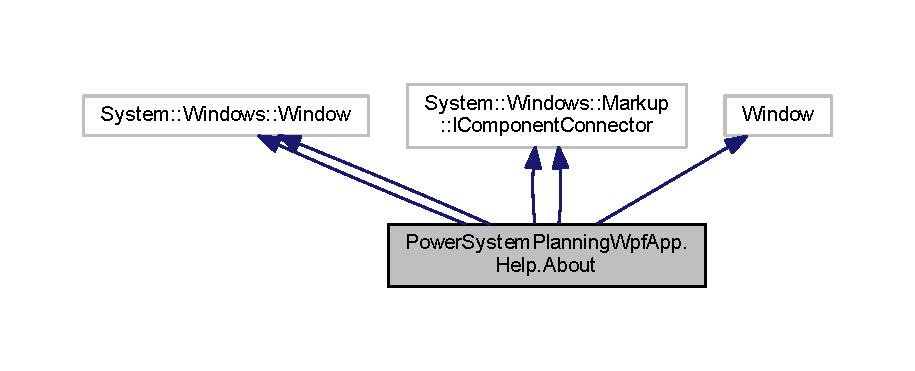
\includegraphics[width=350pt]{class_power_system_planning_wpf_app_1_1_help_1_1_about__inherit__graph}
\end{center}
\end{figure}


Collaboration diagram for Power\+System\+Planning\+Wpf\+App.\+Help.\+About\+:\nopagebreak
\begin{figure}[H]
\begin{center}
\leavevmode
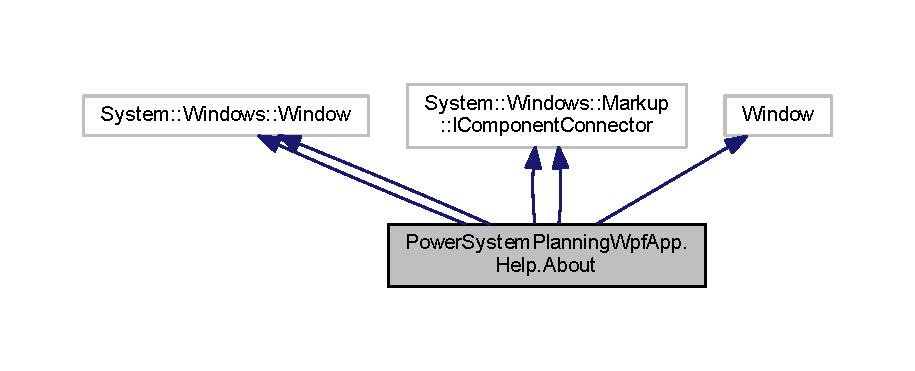
\includegraphics[width=350pt]{class_power_system_planning_wpf_app_1_1_help_1_1_about__coll__graph}
\end{center}
\end{figure}
\subsection*{Public Member Functions}
\begin{DoxyCompactItemize}
\item 
void \hyperlink{class_power_system_planning_wpf_app_1_1_help_1_1_about_a3e07271b4e0d2bf41bff4947516b72e7}{Initialize\+Component} ()
\begin{DoxyCompactList}\small\item\em Initialize\+Component \end{DoxyCompactList}\item 
void \hyperlink{class_power_system_planning_wpf_app_1_1_help_1_1_about_a3e07271b4e0d2bf41bff4947516b72e7}{Initialize\+Component} ()
\begin{DoxyCompactList}\small\item\em Initialize\+Component \end{DoxyCompactList}\end{DoxyCompactItemize}


\subsection{Detailed Description}
Interaction logic for About.\+xaml 

\hyperlink{class_power_system_planning_wpf_app_1_1_help_1_1_about}{About} 

\subsection{Member Function Documentation}
\index{Power\+System\+Planning\+Wpf\+App\+::\+Help\+::\+About@{Power\+System\+Planning\+Wpf\+App\+::\+Help\+::\+About}!Initialize\+Component@{Initialize\+Component}}
\index{Initialize\+Component@{Initialize\+Component}!Power\+System\+Planning\+Wpf\+App\+::\+Help\+::\+About@{Power\+System\+Planning\+Wpf\+App\+::\+Help\+::\+About}}
\subsubsection[{\texorpdfstring{Initialize\+Component()}{InitializeComponent()}}]{\setlength{\rightskip}{0pt plus 5cm}void Power\+System\+Planning\+Wpf\+App.\+Help.\+About.\+Initialize\+Component (
\begin{DoxyParamCaption}
{}
\end{DoxyParamCaption}
)\hspace{0.3cm}{\ttfamily [inline]}}\hypertarget{class_power_system_planning_wpf_app_1_1_help_1_1_about_a3e07271b4e0d2bf41bff4947516b72e7}{}\label{class_power_system_planning_wpf_app_1_1_help_1_1_about_a3e07271b4e0d2bf41bff4947516b72e7}


Initialize\+Component 

\index{Power\+System\+Planning\+Wpf\+App\+::\+Help\+::\+About@{Power\+System\+Planning\+Wpf\+App\+::\+Help\+::\+About}!Initialize\+Component@{Initialize\+Component}}
\index{Initialize\+Component@{Initialize\+Component}!Power\+System\+Planning\+Wpf\+App\+::\+Help\+::\+About@{Power\+System\+Planning\+Wpf\+App\+::\+Help\+::\+About}}
\subsubsection[{\texorpdfstring{Initialize\+Component()}{InitializeComponent()}}]{\setlength{\rightskip}{0pt plus 5cm}void Power\+System\+Planning\+Wpf\+App.\+Help.\+About.\+Initialize\+Component (
\begin{DoxyParamCaption}
{}
\end{DoxyParamCaption}
)\hspace{0.3cm}{\ttfamily [inline]}}\hypertarget{class_power_system_planning_wpf_app_1_1_help_1_1_about_a3e07271b4e0d2bf41bff4947516b72e7}{}\label{class_power_system_planning_wpf_app_1_1_help_1_1_about_a3e07271b4e0d2bf41bff4947516b72e7}


Initialize\+Component 



The documentation for this class was generated from the following files\+:\begin{DoxyCompactItemize}
\item 
Help/About.\+xaml.\+cs\item 
obj/\+Debug/\+Help/About.\+g.\+cs\item 
obj/\+Debug/\+Help/About.\+g.\+i.\+cs\end{DoxyCompactItemize}

\hypertarget{class_power_system_planning_wpf_app_1_1_app}{}\section{Power\+System\+Planning\+Wpf\+App.\+App Class Reference}
\label{class_power_system_planning_wpf_app_1_1_app}\index{Power\+System\+Planning\+Wpf\+App.\+App@{Power\+System\+Planning\+Wpf\+App.\+App}}


Interaction logic for App.\+xaml  




Inheritance diagram for Power\+System\+Planning\+Wpf\+App.\+App\+:\nopagebreak
\begin{figure}[H]
\begin{center}
\leavevmode
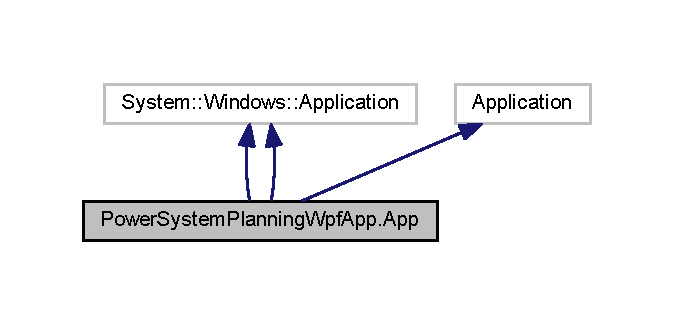
\includegraphics[width=324pt]{class_power_system_planning_wpf_app_1_1_app__inherit__graph}
\end{center}
\end{figure}


Collaboration diagram for Power\+System\+Planning\+Wpf\+App.\+App\+:\nopagebreak
\begin{figure}[H]
\begin{center}
\leavevmode
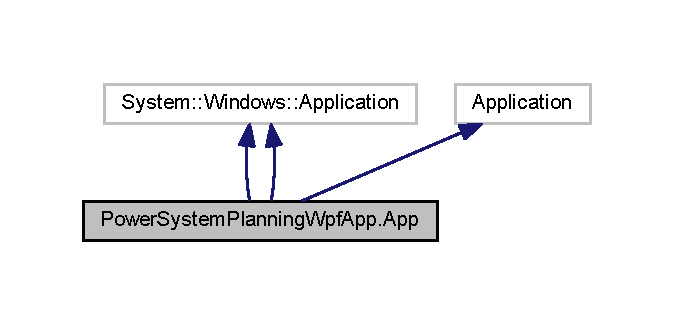
\includegraphics[width=324pt]{class_power_system_planning_wpf_app_1_1_app__coll__graph}
\end{center}
\end{figure}
\subsection*{Public Member Functions}
\begin{DoxyCompactItemize}
\item 
void \hyperlink{class_power_system_planning_wpf_app_1_1_app_abb8be3aedfdf2605dad9e7b85e4db491}{Initialize\+Component} ()
\begin{DoxyCompactList}\small\item\em Initialize\+Component \end{DoxyCompactList}\item 
void \hyperlink{class_power_system_planning_wpf_app_1_1_app_abb8be3aedfdf2605dad9e7b85e4db491}{Initialize\+Component} ()
\begin{DoxyCompactList}\small\item\em Initialize\+Component \end{DoxyCompactList}\end{DoxyCompactItemize}
\subsection*{Static Public Member Functions}
\begin{DoxyCompactItemize}
\item 
static void \hyperlink{class_power_system_planning_wpf_app_1_1_app_aa23fe02d7267383953638c68a677eea8}{Main} ()
\begin{DoxyCompactList}\small\item\em Application Entry Point. \end{DoxyCompactList}\item 
static void \hyperlink{class_power_system_planning_wpf_app_1_1_app_aa23fe02d7267383953638c68a677eea8}{Main} ()
\begin{DoxyCompactList}\small\item\em Application Entry Point. \end{DoxyCompactList}\end{DoxyCompactItemize}


\subsection{Detailed Description}
Interaction logic for App.\+xaml 

\hyperlink{class_power_system_planning_wpf_app_1_1_app}{App} 

\subsection{Member Function Documentation}
\index{Power\+System\+Planning\+Wpf\+App\+::\+App@{Power\+System\+Planning\+Wpf\+App\+::\+App}!Initialize\+Component@{Initialize\+Component}}
\index{Initialize\+Component@{Initialize\+Component}!Power\+System\+Planning\+Wpf\+App\+::\+App@{Power\+System\+Planning\+Wpf\+App\+::\+App}}
\subsubsection[{\texorpdfstring{Initialize\+Component()}{InitializeComponent()}}]{\setlength{\rightskip}{0pt plus 5cm}void Power\+System\+Planning\+Wpf\+App.\+App.\+Initialize\+Component (
\begin{DoxyParamCaption}
{}
\end{DoxyParamCaption}
)\hspace{0.3cm}{\ttfamily [inline]}}\hypertarget{class_power_system_planning_wpf_app_1_1_app_abb8be3aedfdf2605dad9e7b85e4db491}{}\label{class_power_system_planning_wpf_app_1_1_app_abb8be3aedfdf2605dad9e7b85e4db491}


Initialize\+Component 

\index{Power\+System\+Planning\+Wpf\+App\+::\+App@{Power\+System\+Planning\+Wpf\+App\+::\+App}!Initialize\+Component@{Initialize\+Component}}
\index{Initialize\+Component@{Initialize\+Component}!Power\+System\+Planning\+Wpf\+App\+::\+App@{Power\+System\+Planning\+Wpf\+App\+::\+App}}
\subsubsection[{\texorpdfstring{Initialize\+Component()}{InitializeComponent()}}]{\setlength{\rightskip}{0pt plus 5cm}void Power\+System\+Planning\+Wpf\+App.\+App.\+Initialize\+Component (
\begin{DoxyParamCaption}
{}
\end{DoxyParamCaption}
)\hspace{0.3cm}{\ttfamily [inline]}}\hypertarget{class_power_system_planning_wpf_app_1_1_app_abb8be3aedfdf2605dad9e7b85e4db491}{}\label{class_power_system_planning_wpf_app_1_1_app_abb8be3aedfdf2605dad9e7b85e4db491}


Initialize\+Component 

\index{Power\+System\+Planning\+Wpf\+App\+::\+App@{Power\+System\+Planning\+Wpf\+App\+::\+App}!Main@{Main}}
\index{Main@{Main}!Power\+System\+Planning\+Wpf\+App\+::\+App@{Power\+System\+Planning\+Wpf\+App\+::\+App}}
\subsubsection[{\texorpdfstring{Main()}{Main()}}]{\setlength{\rightskip}{0pt plus 5cm}static void Power\+System\+Planning\+Wpf\+App.\+App.\+Main (
\begin{DoxyParamCaption}
{}
\end{DoxyParamCaption}
)\hspace{0.3cm}{\ttfamily [inline]}, {\ttfamily [static]}}\hypertarget{class_power_system_planning_wpf_app_1_1_app_aa23fe02d7267383953638c68a677eea8}{}\label{class_power_system_planning_wpf_app_1_1_app_aa23fe02d7267383953638c68a677eea8}


Application Entry Point. 

\index{Power\+System\+Planning\+Wpf\+App\+::\+App@{Power\+System\+Planning\+Wpf\+App\+::\+App}!Main@{Main}}
\index{Main@{Main}!Power\+System\+Planning\+Wpf\+App\+::\+App@{Power\+System\+Planning\+Wpf\+App\+::\+App}}
\subsubsection[{\texorpdfstring{Main()}{Main()}}]{\setlength{\rightskip}{0pt plus 5cm}static void Power\+System\+Planning\+Wpf\+App.\+App.\+Main (
\begin{DoxyParamCaption}
{}
\end{DoxyParamCaption}
)\hspace{0.3cm}{\ttfamily [inline]}, {\ttfamily [static]}}\hypertarget{class_power_system_planning_wpf_app_1_1_app_aa23fe02d7267383953638c68a677eea8}{}\label{class_power_system_planning_wpf_app_1_1_app_aa23fe02d7267383953638c68a677eea8}


Application Entry Point. 



The documentation for this class was generated from the following files\+:\begin{DoxyCompactItemize}
\item 
App.\+xaml.\+cs\item 
obj/\+Debug/App.\+g.\+cs\item 
obj/\+Debug/App.\+g.\+i.\+cs\end{DoxyCompactItemize}

\hypertarget{class_power_system_planning_wpf_app_1_1_control_utils_1_1_csv_helper}{}\section{Power\+System\+Planning\+Wpf\+App.\+Control\+Utils.\+Csv\+Helper Class Reference}
\label{class_power_system_planning_wpf_app_1_1_control_utils_1_1_csv_helper}\index{Power\+System\+Planning\+Wpf\+App.\+Control\+Utils.\+Csv\+Helper@{Power\+System\+Planning\+Wpf\+App.\+Control\+Utils.\+Csv\+Helper}}
\subsection*{Public Types}
\begin{DoxyCompactItemize}
\item 
enum {\bfseries Line\+Separator} \{ {\bfseries Unknown} = 0, 
{\bfseries Tab}, 
{\bfseries Semicolon}, 
{\bfseries Comma}
 \}\hypertarget{class_power_system_planning_wpf_app_1_1_control_utils_1_1_csv_helper_a70691f6b3ee3b980dfcb2d789e705720}{}\label{class_power_system_planning_wpf_app_1_1_control_utils_1_1_csv_helper_a70691f6b3ee3b980dfcb2d789e705720}

\end{DoxyCompactItemize}
\subsection*{Static Public Member Functions}
\begin{DoxyCompactItemize}
\item 
static Line\+Separator {\bfseries Guess\+Csv\+Separator} (string one\+Line)\hypertarget{class_power_system_planning_wpf_app_1_1_control_utils_1_1_csv_helper_ae65843294e79ea18500e5e4e0f54e50b}{}\label{class_power_system_planning_wpf_app_1_1_control_utils_1_1_csv_helper_ae65843294e79ea18500e5e4e0f54e50b}

\item 
static string\mbox{[}$\,$\mbox{]} {\bfseries Parse\+Line\+Comma\+Separated} (string line)\hypertarget{class_power_system_planning_wpf_app_1_1_control_utils_1_1_csv_helper_ae308762112aa7269bfa184769481a115}{}\label{class_power_system_planning_wpf_app_1_1_control_utils_1_1_csv_helper_ae308762112aa7269bfa184769481a115}

\item 
static string\mbox{[}$\,$\mbox{]} {\bfseries Parse\+Line\+Tab\+Separated} (string line)\hypertarget{class_power_system_planning_wpf_app_1_1_control_utils_1_1_csv_helper_a4654fa5f46540d5f8d3ad315e67fe85b}{}\label{class_power_system_planning_wpf_app_1_1_control_utils_1_1_csv_helper_a4654fa5f46540d5f8d3ad315e67fe85b}

\item 
static string\mbox{[}$\,$\mbox{]} {\bfseries Parse\+Line\+Semicolon\+Separated} (string line)\hypertarget{class_power_system_planning_wpf_app_1_1_control_utils_1_1_csv_helper_aa72cbd39b41c688fcf99011b50de7dbc}{}\label{class_power_system_planning_wpf_app_1_1_control_utils_1_1_csv_helper_aa72cbd39b41c688fcf99011b50de7dbc}

\item 
static string\mbox{[}$\,$\mbox{]} {\bfseries Parse\+Line\+Not\+Separated} (string line)\hypertarget{class_power_system_planning_wpf_app_1_1_control_utils_1_1_csv_helper_a8b8b2eca8cf0b1d3e8d58ca6948c6e5e}{}\label{class_power_system_planning_wpf_app_1_1_control_utils_1_1_csv_helper_a8b8b2eca8cf0b1d3e8d58ca6948c6e5e}

\item 
static List$<$ string\mbox{[}$\,$\mbox{]}$>$ {\bfseries Parse\+Text} (string text)\hypertarget{class_power_system_planning_wpf_app_1_1_control_utils_1_1_csv_helper_a6c4a431b2380a4d6b779ec4869a25b10}{}\label{class_power_system_planning_wpf_app_1_1_control_utils_1_1_csv_helper_a6c4a431b2380a4d6b779ec4869a25b10}

\item 
static List$<$ string\mbox{[}$\,$\mbox{]}$>$ {\bfseries Parse\+String} (string\mbox{[}$\,$\mbox{]} lines)\hypertarget{class_power_system_planning_wpf_app_1_1_control_utils_1_1_csv_helper_abfb8964ea9c48762b9c994280d38bc6f}{}\label{class_power_system_planning_wpf_app_1_1_control_utils_1_1_csv_helper_abfb8964ea9c48762b9c994280d38bc6f}

\end{DoxyCompactItemize}
\subsection*{Static Public Attributes}
\begin{DoxyCompactItemize}
\item 
static Dictionary$<$ Line\+Separator, Func$<$ string, string\mbox{[}$\,$\mbox{]}$>$ $>$ {\bfseries Dictionary\+Of\+Line\+Separator\+And\+Its\+Func} = new Dictionary$<$Line\+Separator, Func$<$string, string\mbox{[}$\,$\mbox{]}$>$$>$()\hypertarget{class_power_system_planning_wpf_app_1_1_control_utils_1_1_csv_helper_a857e4da4f229926717b5fa8f28fab105}{}\label{class_power_system_planning_wpf_app_1_1_control_utils_1_1_csv_helper_a857e4da4f229926717b5fa8f28fab105}

\end{DoxyCompactItemize}


The documentation for this class was generated from the following file\+:\begin{DoxyCompactItemize}
\item 
Control\+Utils/Csv\+Helper.\+cs\end{DoxyCompactItemize}

\hypertarget{class_power_system_planning_wpf_app_1_1_control_utils_1_1_custom_data_grid}{}\section{Power\+System\+Planning\+Wpf\+App.\+Control\+Utils.\+Custom\+Data\+Grid Class Reference}
\label{class_power_system_planning_wpf_app_1_1_control_utils_1_1_custom_data_grid}\index{Power\+System\+Planning\+Wpf\+App.\+Control\+Utils.\+Custom\+Data\+Grid@{Power\+System\+Planning\+Wpf\+App.\+Control\+Utils.\+Custom\+Data\+Grid}}


Inheritance diagram for Power\+System\+Planning\+Wpf\+App.\+Control\+Utils.\+Custom\+Data\+Grid\+:\nopagebreak
\begin{figure}[H]
\begin{center}
\leavevmode
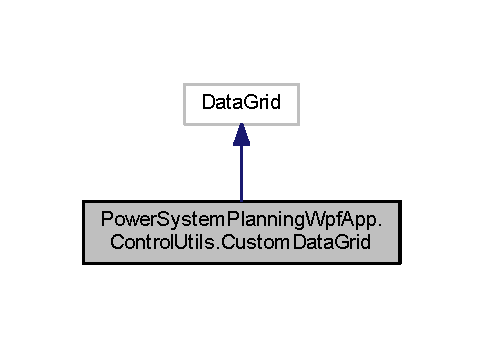
\includegraphics[width=232pt]{class_power_system_planning_wpf_app_1_1_control_utils_1_1_custom_data_grid__inherit__graph}
\end{center}
\end{figure}


Collaboration diagram for Power\+System\+Planning\+Wpf\+App.\+Control\+Utils.\+Custom\+Data\+Grid\+:\nopagebreak
\begin{figure}[H]
\begin{center}
\leavevmode
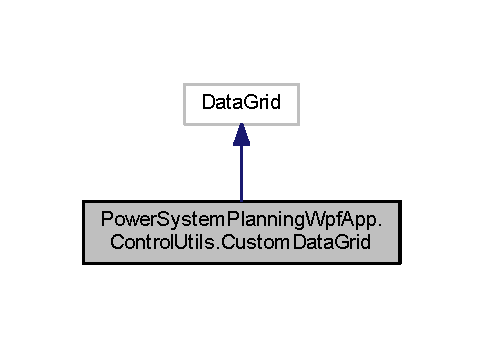
\includegraphics[width=232pt]{class_power_system_planning_wpf_app_1_1_control_utils_1_1_custom_data_grid__coll__graph}
\end{center}
\end{figure}
\subsection*{Public Member Functions}
\begin{DoxyCompactItemize}
\item 
void {\bfseries Set\+Grid\+Writable\+Ex} ()\hypertarget{class_power_system_planning_wpf_app_1_1_control_utils_1_1_custom_data_grid_acbd04f519f5b4788fc8a9699bb005d04}{}\label{class_power_system_planning_wpf_app_1_1_control_utils_1_1_custom_data_grid_acbd04f519f5b4788fc8a9699bb005d04}

\end{DoxyCompactItemize}
\subsection*{Static Public Attributes}
\begin{DoxyCompactItemize}
\item 
static readonly Dependency\+Property \hyperlink{class_power_system_planning_wpf_app_1_1_control_utils_1_1_custom_data_grid_a2521d8f0307ab66a4fa0c1c31c305332}{Can\+User\+Paste\+To\+New\+Rows\+Property}
\begin{DoxyCompactList}\small\item\em Dependency\+Property for Can\+User\+Add\+Rows. \end{DoxyCompactList}\end{DoxyCompactItemize}
\subsection*{Protected Member Functions}
\begin{DoxyCompactItemize}
\item 
virtual void \hyperlink{class_power_system_planning_wpf_app_1_1_control_utils_1_1_custom_data_grid_ad62754f9382daa406815f7965d6af785}{On\+Can\+Execute\+Paste} (object target, Can\+Execute\+Routed\+Event\+Args args)
\begin{DoxyCompactList}\small\item\em This virtual method is called when Application\+Commands.\+Paste command query its state. \end{DoxyCompactList}\item 
virtual void \hyperlink{class_power_system_planning_wpf_app_1_1_control_utils_1_1_custom_data_grid_a7a8455f1c46a856165914960a0e60418}{On\+Executed\+Paste} (object target, Executed\+Routed\+Event\+Args args)
\begin{DoxyCompactList}\small\item\em This virtual method is called when Application\+Commands.\+Paste command is executed. \end{DoxyCompactList}\end{DoxyCompactItemize}
\subsection*{Properties}
\begin{DoxyCompactItemize}
\item 
bool \hyperlink{class_power_system_planning_wpf_app_1_1_control_utils_1_1_custom_data_grid_a3444d83edb40c95ccf9aca14ffe6f3ce}{Can\+User\+Paste\+To\+New\+Rows}\hspace{0.3cm}{\ttfamily  \mbox{[}get, set\mbox{]}}
\begin{DoxyCompactList}\small\item\em Whether the end-\/user can add new rows to the Items\+Source. \end{DoxyCompactList}\end{DoxyCompactItemize}
\subsection*{Events}
\begin{DoxyCompactItemize}
\item 
Executed\+Routed\+Event\+Handler {\bfseries Execute\+Paste\+Event}\hypertarget{class_power_system_planning_wpf_app_1_1_control_utils_1_1_custom_data_grid_a221845278a5720637f3018528b55a841}{}\label{class_power_system_planning_wpf_app_1_1_control_utils_1_1_custom_data_grid_a221845278a5720637f3018528b55a841}

\item 
Can\+Execute\+Routed\+Event\+Handler {\bfseries Can\+Execute\+Paste\+Event}\hypertarget{class_power_system_planning_wpf_app_1_1_control_utils_1_1_custom_data_grid_abdc4b5da0ef2b3b3f2a36ce995d2d313}{}\label{class_power_system_planning_wpf_app_1_1_control_utils_1_1_custom_data_grid_abdc4b5da0ef2b3b3f2a36ce995d2d313}

\end{DoxyCompactItemize}


\subsection{Member Function Documentation}
\index{Power\+System\+Planning\+Wpf\+App\+::\+Control\+Utils\+::\+Custom\+Data\+Grid@{Power\+System\+Planning\+Wpf\+App\+::\+Control\+Utils\+::\+Custom\+Data\+Grid}!On\+Can\+Execute\+Paste@{On\+Can\+Execute\+Paste}}
\index{On\+Can\+Execute\+Paste@{On\+Can\+Execute\+Paste}!Power\+System\+Planning\+Wpf\+App\+::\+Control\+Utils\+::\+Custom\+Data\+Grid@{Power\+System\+Planning\+Wpf\+App\+::\+Control\+Utils\+::\+Custom\+Data\+Grid}}
\subsubsection[{\texorpdfstring{On\+Can\+Execute\+Paste(object target, Can\+Execute\+Routed\+Event\+Args args)}{OnCanExecutePaste(object target, CanExecuteRoutedEventArgs args)}}]{\setlength{\rightskip}{0pt plus 5cm}virtual void Power\+System\+Planning\+Wpf\+App.\+Control\+Utils.\+Custom\+Data\+Grid.\+On\+Can\+Execute\+Paste (
\begin{DoxyParamCaption}
\item[{object}]{target, }
\item[{Can\+Execute\+Routed\+Event\+Args}]{args}
\end{DoxyParamCaption}
)\hspace{0.3cm}{\ttfamily [inline]}, {\ttfamily [protected]}, {\ttfamily [virtual]}}\hypertarget{class_power_system_planning_wpf_app_1_1_control_utils_1_1_custom_data_grid_ad62754f9382daa406815f7965d6af785}{}\label{class_power_system_planning_wpf_app_1_1_control_utils_1_1_custom_data_grid_ad62754f9382daa406815f7965d6af785}


This virtual method is called when Application\+Commands.\+Paste command query its state. 


\begin{DoxyParams}{Parameters}
{\em args} & \\
\hline
\end{DoxyParams}
\index{Power\+System\+Planning\+Wpf\+App\+::\+Control\+Utils\+::\+Custom\+Data\+Grid@{Power\+System\+Planning\+Wpf\+App\+::\+Control\+Utils\+::\+Custom\+Data\+Grid}!On\+Executed\+Paste@{On\+Executed\+Paste}}
\index{On\+Executed\+Paste@{On\+Executed\+Paste}!Power\+System\+Planning\+Wpf\+App\+::\+Control\+Utils\+::\+Custom\+Data\+Grid@{Power\+System\+Planning\+Wpf\+App\+::\+Control\+Utils\+::\+Custom\+Data\+Grid}}
\subsubsection[{\texorpdfstring{On\+Executed\+Paste(object target, Executed\+Routed\+Event\+Args args)}{OnExecutedPaste(object target, ExecutedRoutedEventArgs args)}}]{\setlength{\rightskip}{0pt plus 5cm}virtual void Power\+System\+Planning\+Wpf\+App.\+Control\+Utils.\+Custom\+Data\+Grid.\+On\+Executed\+Paste (
\begin{DoxyParamCaption}
\item[{object}]{target, }
\item[{Executed\+Routed\+Event\+Args}]{args}
\end{DoxyParamCaption}
)\hspace{0.3cm}{\ttfamily [inline]}, {\ttfamily [protected]}, {\ttfamily [virtual]}}\hypertarget{class_power_system_planning_wpf_app_1_1_control_utils_1_1_custom_data_grid_a7a8455f1c46a856165914960a0e60418}{}\label{class_power_system_planning_wpf_app_1_1_control_utils_1_1_custom_data_grid_a7a8455f1c46a856165914960a0e60418}


This virtual method is called when Application\+Commands.\+Paste command is executed. 


\begin{DoxyParams}{Parameters}
{\em target} & \\
\hline
{\em args} & \\
\hline
\end{DoxyParams}


\subsection{Member Data Documentation}
\index{Power\+System\+Planning\+Wpf\+App\+::\+Control\+Utils\+::\+Custom\+Data\+Grid@{Power\+System\+Planning\+Wpf\+App\+::\+Control\+Utils\+::\+Custom\+Data\+Grid}!Can\+User\+Paste\+To\+New\+Rows\+Property@{Can\+User\+Paste\+To\+New\+Rows\+Property}}
\index{Can\+User\+Paste\+To\+New\+Rows\+Property@{Can\+User\+Paste\+To\+New\+Rows\+Property}!Power\+System\+Planning\+Wpf\+App\+::\+Control\+Utils\+::\+Custom\+Data\+Grid@{Power\+System\+Planning\+Wpf\+App\+::\+Control\+Utils\+::\+Custom\+Data\+Grid}}
\subsubsection[{\texorpdfstring{Can\+User\+Paste\+To\+New\+Rows\+Property}{CanUserPasteToNewRowsProperty}}]{\setlength{\rightskip}{0pt plus 5cm}readonly Dependency\+Property Power\+System\+Planning\+Wpf\+App.\+Control\+Utils.\+Custom\+Data\+Grid.\+Can\+User\+Paste\+To\+New\+Rows\+Property\hspace{0.3cm}{\ttfamily [static]}}\hypertarget{class_power_system_planning_wpf_app_1_1_control_utils_1_1_custom_data_grid_a2521d8f0307ab66a4fa0c1c31c305332}{}\label{class_power_system_planning_wpf_app_1_1_control_utils_1_1_custom_data_grid_a2521d8f0307ab66a4fa0c1c31c305332}
{\bfseries Initial value\+:}
\begin{DoxyCode}
=
            DependencyProperty.Register(\textcolor{stringliteral}{"CanUserPasteToNewRows"},
                                        typeof(\textcolor{keywordtype}{bool}), typeof(CustomDataGrid),
                                        \textcolor{keyword}{new} FrameworkPropertyMetadata(\textcolor{keyword}{true}, null, null))
\end{DoxyCode}


Dependency\+Property for Can\+User\+Add\+Rows. 



\subsection{Property Documentation}
\index{Power\+System\+Planning\+Wpf\+App\+::\+Control\+Utils\+::\+Custom\+Data\+Grid@{Power\+System\+Planning\+Wpf\+App\+::\+Control\+Utils\+::\+Custom\+Data\+Grid}!Can\+User\+Paste\+To\+New\+Rows@{Can\+User\+Paste\+To\+New\+Rows}}
\index{Can\+User\+Paste\+To\+New\+Rows@{Can\+User\+Paste\+To\+New\+Rows}!Power\+System\+Planning\+Wpf\+App\+::\+Control\+Utils\+::\+Custom\+Data\+Grid@{Power\+System\+Planning\+Wpf\+App\+::\+Control\+Utils\+::\+Custom\+Data\+Grid}}
\subsubsection[{\texorpdfstring{Can\+User\+Paste\+To\+New\+Rows}{CanUserPasteToNewRows}}]{\setlength{\rightskip}{0pt plus 5cm}bool Power\+System\+Planning\+Wpf\+App.\+Control\+Utils.\+Custom\+Data\+Grid.\+Can\+User\+Paste\+To\+New\+Rows\hspace{0.3cm}{\ttfamily [get]}, {\ttfamily [set]}}\hypertarget{class_power_system_planning_wpf_app_1_1_control_utils_1_1_custom_data_grid_a3444d83edb40c95ccf9aca14ffe6f3ce}{}\label{class_power_system_planning_wpf_app_1_1_control_utils_1_1_custom_data_grid_a3444d83edb40c95ccf9aca14ffe6f3ce}


Whether the end-\/user can add new rows to the Items\+Source. 



The documentation for this class was generated from the following file\+:\begin{DoxyCompactItemize}
\item 
Control\+Utils/Custom\+Data\+Grid.\+cs\end{DoxyCompactItemize}

\input{class_power_system_planning_wpf_app_1_1_control_utils_1_1_datagrid_test}
\hypertarget{class_xaml_generated_namespace_1_1_generated_internal_type_helper}{}\section{Xaml\+Generated\+Namespace.\+Generated\+Internal\+Type\+Helper Class Reference}
\label{class_xaml_generated_namespace_1_1_generated_internal_type_helper}\index{Xaml\+Generated\+Namespace.\+Generated\+Internal\+Type\+Helper@{Xaml\+Generated\+Namespace.\+Generated\+Internal\+Type\+Helper}}


\hyperlink{class_xaml_generated_namespace_1_1_generated_internal_type_helper}{Generated\+Internal\+Type\+Helper}  




Inheritance diagram for Xaml\+Generated\+Namespace.\+Generated\+Internal\+Type\+Helper\+:\nopagebreak
\begin{figure}[H]
\begin{center}
\leavevmode
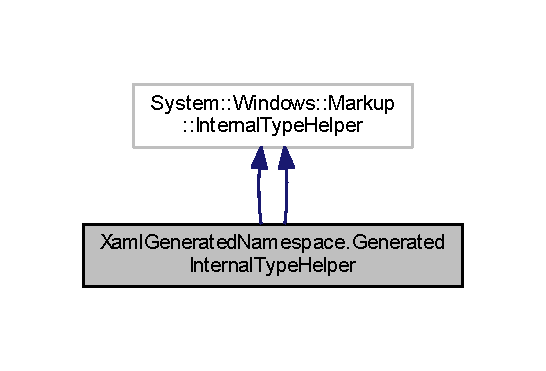
\includegraphics[width=262pt]{class_xaml_generated_namespace_1_1_generated_internal_type_helper__inherit__graph}
\end{center}
\end{figure}


Collaboration diagram for Xaml\+Generated\+Namespace.\+Generated\+Internal\+Type\+Helper\+:\nopagebreak
\begin{figure}[H]
\begin{center}
\leavevmode
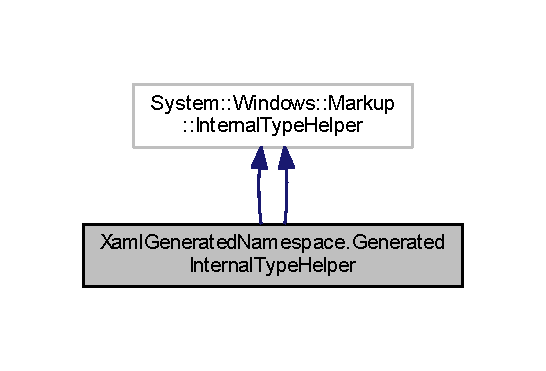
\includegraphics[width=262pt]{class_xaml_generated_namespace_1_1_generated_internal_type_helper__coll__graph}
\end{center}
\end{figure}
\subsection*{Protected Member Functions}
\begin{DoxyCompactItemize}
\item 
override object \hyperlink{class_xaml_generated_namespace_1_1_generated_internal_type_helper_aefb7a98fceb9c287cef4756942f441d1}{Create\+Instance} (System.\+Type type, System.\+Globalization.\+Culture\+Info culture)
\begin{DoxyCompactList}\small\item\em Create\+Instance \end{DoxyCompactList}\item 
override object \hyperlink{class_xaml_generated_namespace_1_1_generated_internal_type_helper_afdc9fe15b56607d02082908d934480c6}{Get\+Property\+Value} (System.\+Reflection.\+Property\+Info property\+Info, object target, System.\+Globalization.\+Culture\+Info culture)
\begin{DoxyCompactList}\small\item\em Get\+Property\+Value \end{DoxyCompactList}\item 
override void \hyperlink{class_xaml_generated_namespace_1_1_generated_internal_type_helper_ade0f04c0f7b18dd5b170e071d5534d38}{Set\+Property\+Value} (System.\+Reflection.\+Property\+Info property\+Info, object target, object value, System.\+Globalization.\+Culture\+Info culture)
\begin{DoxyCompactList}\small\item\em Set\+Property\+Value \end{DoxyCompactList}\item 
override System.\+Delegate \hyperlink{class_xaml_generated_namespace_1_1_generated_internal_type_helper_a8ec4c37e82d9f4e867e9655f4eac3a78}{Create\+Delegate} (System.\+Type delegate\+Type, object target, string handler)
\begin{DoxyCompactList}\small\item\em Create\+Delegate \end{DoxyCompactList}\item 
override void \hyperlink{class_xaml_generated_namespace_1_1_generated_internal_type_helper_a73471f4a6d1ca4c4fceec9ad8610f0c8}{Add\+Event\+Handler} (System.\+Reflection.\+Event\+Info event\+Info, object target, System.\+Delegate handler)
\begin{DoxyCompactList}\small\item\em Add\+Event\+Handler \end{DoxyCompactList}\item 
override object \hyperlink{class_xaml_generated_namespace_1_1_generated_internal_type_helper_aefb7a98fceb9c287cef4756942f441d1}{Create\+Instance} (System.\+Type type, System.\+Globalization.\+Culture\+Info culture)
\begin{DoxyCompactList}\small\item\em Create\+Instance \end{DoxyCompactList}\item 
override object \hyperlink{class_xaml_generated_namespace_1_1_generated_internal_type_helper_afdc9fe15b56607d02082908d934480c6}{Get\+Property\+Value} (System.\+Reflection.\+Property\+Info property\+Info, object target, System.\+Globalization.\+Culture\+Info culture)
\begin{DoxyCompactList}\small\item\em Get\+Property\+Value \end{DoxyCompactList}\item 
override void \hyperlink{class_xaml_generated_namespace_1_1_generated_internal_type_helper_ade0f04c0f7b18dd5b170e071d5534d38}{Set\+Property\+Value} (System.\+Reflection.\+Property\+Info property\+Info, object target, object value, System.\+Globalization.\+Culture\+Info culture)
\begin{DoxyCompactList}\small\item\em Set\+Property\+Value \end{DoxyCompactList}\item 
override System.\+Delegate \hyperlink{class_xaml_generated_namespace_1_1_generated_internal_type_helper_a8ec4c37e82d9f4e867e9655f4eac3a78}{Create\+Delegate} (System.\+Type delegate\+Type, object target, string handler)
\begin{DoxyCompactList}\small\item\em Create\+Delegate \end{DoxyCompactList}\item 
override void \hyperlink{class_xaml_generated_namespace_1_1_generated_internal_type_helper_a73471f4a6d1ca4c4fceec9ad8610f0c8}{Add\+Event\+Handler} (System.\+Reflection.\+Event\+Info event\+Info, object target, System.\+Delegate handler)
\begin{DoxyCompactList}\small\item\em Add\+Event\+Handler \end{DoxyCompactList}\end{DoxyCompactItemize}


\subsection{Detailed Description}
\hyperlink{class_xaml_generated_namespace_1_1_generated_internal_type_helper}{Generated\+Internal\+Type\+Helper} 



\subsection{Member Function Documentation}
\index{Xaml\+Generated\+Namespace\+::\+Generated\+Internal\+Type\+Helper@{Xaml\+Generated\+Namespace\+::\+Generated\+Internal\+Type\+Helper}!Add\+Event\+Handler@{Add\+Event\+Handler}}
\index{Add\+Event\+Handler@{Add\+Event\+Handler}!Xaml\+Generated\+Namespace\+::\+Generated\+Internal\+Type\+Helper@{Xaml\+Generated\+Namespace\+::\+Generated\+Internal\+Type\+Helper}}
\subsubsection[{\texorpdfstring{Add\+Event\+Handler(\+System.\+Reflection.\+Event\+Info event\+Info, object target, System.\+Delegate handler)}{AddEventHandler(System.Reflection.EventInfo eventInfo, object target, System.Delegate handler)}}]{\setlength{\rightskip}{0pt plus 5cm}override void Xaml\+Generated\+Namespace.\+Generated\+Internal\+Type\+Helper.\+Add\+Event\+Handler (
\begin{DoxyParamCaption}
\item[{System.\+Reflection.\+Event\+Info}]{event\+Info, }
\item[{object}]{target, }
\item[{System.\+Delegate}]{handler}
\end{DoxyParamCaption}
)\hspace{0.3cm}{\ttfamily [inline]}, {\ttfamily [protected]}}\hypertarget{class_xaml_generated_namespace_1_1_generated_internal_type_helper_a73471f4a6d1ca4c4fceec9ad8610f0c8}{}\label{class_xaml_generated_namespace_1_1_generated_internal_type_helper_a73471f4a6d1ca4c4fceec9ad8610f0c8}


Add\+Event\+Handler 

\index{Xaml\+Generated\+Namespace\+::\+Generated\+Internal\+Type\+Helper@{Xaml\+Generated\+Namespace\+::\+Generated\+Internal\+Type\+Helper}!Add\+Event\+Handler@{Add\+Event\+Handler}}
\index{Add\+Event\+Handler@{Add\+Event\+Handler}!Xaml\+Generated\+Namespace\+::\+Generated\+Internal\+Type\+Helper@{Xaml\+Generated\+Namespace\+::\+Generated\+Internal\+Type\+Helper}}
\subsubsection[{\texorpdfstring{Add\+Event\+Handler(\+System.\+Reflection.\+Event\+Info event\+Info, object target, System.\+Delegate handler)}{AddEventHandler(System.Reflection.EventInfo eventInfo, object target, System.Delegate handler)}}]{\setlength{\rightskip}{0pt plus 5cm}override void Xaml\+Generated\+Namespace.\+Generated\+Internal\+Type\+Helper.\+Add\+Event\+Handler (
\begin{DoxyParamCaption}
\item[{System.\+Reflection.\+Event\+Info}]{event\+Info, }
\item[{object}]{target, }
\item[{System.\+Delegate}]{handler}
\end{DoxyParamCaption}
)\hspace{0.3cm}{\ttfamily [inline]}, {\ttfamily [protected]}}\hypertarget{class_xaml_generated_namespace_1_1_generated_internal_type_helper_a73471f4a6d1ca4c4fceec9ad8610f0c8}{}\label{class_xaml_generated_namespace_1_1_generated_internal_type_helper_a73471f4a6d1ca4c4fceec9ad8610f0c8}


Add\+Event\+Handler 

\index{Xaml\+Generated\+Namespace\+::\+Generated\+Internal\+Type\+Helper@{Xaml\+Generated\+Namespace\+::\+Generated\+Internal\+Type\+Helper}!Create\+Delegate@{Create\+Delegate}}
\index{Create\+Delegate@{Create\+Delegate}!Xaml\+Generated\+Namespace\+::\+Generated\+Internal\+Type\+Helper@{Xaml\+Generated\+Namespace\+::\+Generated\+Internal\+Type\+Helper}}
\subsubsection[{\texorpdfstring{Create\+Delegate(\+System.\+Type delegate\+Type, object target, string handler)}{CreateDelegate(System.Type delegateType, object target, string handler)}}]{\setlength{\rightskip}{0pt plus 5cm}override System.\+Delegate Xaml\+Generated\+Namespace.\+Generated\+Internal\+Type\+Helper.\+Create\+Delegate (
\begin{DoxyParamCaption}
\item[{System.\+Type}]{delegate\+Type, }
\item[{object}]{target, }
\item[{string}]{handler}
\end{DoxyParamCaption}
)\hspace{0.3cm}{\ttfamily [inline]}, {\ttfamily [protected]}}\hypertarget{class_xaml_generated_namespace_1_1_generated_internal_type_helper_a8ec4c37e82d9f4e867e9655f4eac3a78}{}\label{class_xaml_generated_namespace_1_1_generated_internal_type_helper_a8ec4c37e82d9f4e867e9655f4eac3a78}


Create\+Delegate 

\index{Xaml\+Generated\+Namespace\+::\+Generated\+Internal\+Type\+Helper@{Xaml\+Generated\+Namespace\+::\+Generated\+Internal\+Type\+Helper}!Create\+Delegate@{Create\+Delegate}}
\index{Create\+Delegate@{Create\+Delegate}!Xaml\+Generated\+Namespace\+::\+Generated\+Internal\+Type\+Helper@{Xaml\+Generated\+Namespace\+::\+Generated\+Internal\+Type\+Helper}}
\subsubsection[{\texorpdfstring{Create\+Delegate(\+System.\+Type delegate\+Type, object target, string handler)}{CreateDelegate(System.Type delegateType, object target, string handler)}}]{\setlength{\rightskip}{0pt plus 5cm}override System.\+Delegate Xaml\+Generated\+Namespace.\+Generated\+Internal\+Type\+Helper.\+Create\+Delegate (
\begin{DoxyParamCaption}
\item[{System.\+Type}]{delegate\+Type, }
\item[{object}]{target, }
\item[{string}]{handler}
\end{DoxyParamCaption}
)\hspace{0.3cm}{\ttfamily [inline]}, {\ttfamily [protected]}}\hypertarget{class_xaml_generated_namespace_1_1_generated_internal_type_helper_a8ec4c37e82d9f4e867e9655f4eac3a78}{}\label{class_xaml_generated_namespace_1_1_generated_internal_type_helper_a8ec4c37e82d9f4e867e9655f4eac3a78}


Create\+Delegate 

\index{Xaml\+Generated\+Namespace\+::\+Generated\+Internal\+Type\+Helper@{Xaml\+Generated\+Namespace\+::\+Generated\+Internal\+Type\+Helper}!Create\+Instance@{Create\+Instance}}
\index{Create\+Instance@{Create\+Instance}!Xaml\+Generated\+Namespace\+::\+Generated\+Internal\+Type\+Helper@{Xaml\+Generated\+Namespace\+::\+Generated\+Internal\+Type\+Helper}}
\subsubsection[{\texorpdfstring{Create\+Instance(\+System.\+Type type, System.\+Globalization.\+Culture\+Info culture)}{CreateInstance(System.Type type, System.Globalization.CultureInfo culture)}}]{\setlength{\rightskip}{0pt plus 5cm}override object Xaml\+Generated\+Namespace.\+Generated\+Internal\+Type\+Helper.\+Create\+Instance (
\begin{DoxyParamCaption}
\item[{System.\+Type}]{type, }
\item[{System.\+Globalization.\+Culture\+Info}]{culture}
\end{DoxyParamCaption}
)\hspace{0.3cm}{\ttfamily [inline]}, {\ttfamily [protected]}}\hypertarget{class_xaml_generated_namespace_1_1_generated_internal_type_helper_aefb7a98fceb9c287cef4756942f441d1}{}\label{class_xaml_generated_namespace_1_1_generated_internal_type_helper_aefb7a98fceb9c287cef4756942f441d1}


Create\+Instance 

\index{Xaml\+Generated\+Namespace\+::\+Generated\+Internal\+Type\+Helper@{Xaml\+Generated\+Namespace\+::\+Generated\+Internal\+Type\+Helper}!Create\+Instance@{Create\+Instance}}
\index{Create\+Instance@{Create\+Instance}!Xaml\+Generated\+Namespace\+::\+Generated\+Internal\+Type\+Helper@{Xaml\+Generated\+Namespace\+::\+Generated\+Internal\+Type\+Helper}}
\subsubsection[{\texorpdfstring{Create\+Instance(\+System.\+Type type, System.\+Globalization.\+Culture\+Info culture)}{CreateInstance(System.Type type, System.Globalization.CultureInfo culture)}}]{\setlength{\rightskip}{0pt plus 5cm}override object Xaml\+Generated\+Namespace.\+Generated\+Internal\+Type\+Helper.\+Create\+Instance (
\begin{DoxyParamCaption}
\item[{System.\+Type}]{type, }
\item[{System.\+Globalization.\+Culture\+Info}]{culture}
\end{DoxyParamCaption}
)\hspace{0.3cm}{\ttfamily [inline]}, {\ttfamily [protected]}}\hypertarget{class_xaml_generated_namespace_1_1_generated_internal_type_helper_aefb7a98fceb9c287cef4756942f441d1}{}\label{class_xaml_generated_namespace_1_1_generated_internal_type_helper_aefb7a98fceb9c287cef4756942f441d1}


Create\+Instance 

\index{Xaml\+Generated\+Namespace\+::\+Generated\+Internal\+Type\+Helper@{Xaml\+Generated\+Namespace\+::\+Generated\+Internal\+Type\+Helper}!Get\+Property\+Value@{Get\+Property\+Value}}
\index{Get\+Property\+Value@{Get\+Property\+Value}!Xaml\+Generated\+Namespace\+::\+Generated\+Internal\+Type\+Helper@{Xaml\+Generated\+Namespace\+::\+Generated\+Internal\+Type\+Helper}}
\subsubsection[{\texorpdfstring{Get\+Property\+Value(\+System.\+Reflection.\+Property\+Info property\+Info, object target, System.\+Globalization.\+Culture\+Info culture)}{GetPropertyValue(System.Reflection.PropertyInfo propertyInfo, object target, System.Globalization.CultureInfo culture)}}]{\setlength{\rightskip}{0pt plus 5cm}override object Xaml\+Generated\+Namespace.\+Generated\+Internal\+Type\+Helper.\+Get\+Property\+Value (
\begin{DoxyParamCaption}
\item[{System.\+Reflection.\+Property\+Info}]{property\+Info, }
\item[{object}]{target, }
\item[{System.\+Globalization.\+Culture\+Info}]{culture}
\end{DoxyParamCaption}
)\hspace{0.3cm}{\ttfamily [inline]}, {\ttfamily [protected]}}\hypertarget{class_xaml_generated_namespace_1_1_generated_internal_type_helper_afdc9fe15b56607d02082908d934480c6}{}\label{class_xaml_generated_namespace_1_1_generated_internal_type_helper_afdc9fe15b56607d02082908d934480c6}


Get\+Property\+Value 

\index{Xaml\+Generated\+Namespace\+::\+Generated\+Internal\+Type\+Helper@{Xaml\+Generated\+Namespace\+::\+Generated\+Internal\+Type\+Helper}!Get\+Property\+Value@{Get\+Property\+Value}}
\index{Get\+Property\+Value@{Get\+Property\+Value}!Xaml\+Generated\+Namespace\+::\+Generated\+Internal\+Type\+Helper@{Xaml\+Generated\+Namespace\+::\+Generated\+Internal\+Type\+Helper}}
\subsubsection[{\texorpdfstring{Get\+Property\+Value(\+System.\+Reflection.\+Property\+Info property\+Info, object target, System.\+Globalization.\+Culture\+Info culture)}{GetPropertyValue(System.Reflection.PropertyInfo propertyInfo, object target, System.Globalization.CultureInfo culture)}}]{\setlength{\rightskip}{0pt plus 5cm}override object Xaml\+Generated\+Namespace.\+Generated\+Internal\+Type\+Helper.\+Get\+Property\+Value (
\begin{DoxyParamCaption}
\item[{System.\+Reflection.\+Property\+Info}]{property\+Info, }
\item[{object}]{target, }
\item[{System.\+Globalization.\+Culture\+Info}]{culture}
\end{DoxyParamCaption}
)\hspace{0.3cm}{\ttfamily [inline]}, {\ttfamily [protected]}}\hypertarget{class_xaml_generated_namespace_1_1_generated_internal_type_helper_afdc9fe15b56607d02082908d934480c6}{}\label{class_xaml_generated_namespace_1_1_generated_internal_type_helper_afdc9fe15b56607d02082908d934480c6}


Get\+Property\+Value 

\index{Xaml\+Generated\+Namespace\+::\+Generated\+Internal\+Type\+Helper@{Xaml\+Generated\+Namespace\+::\+Generated\+Internal\+Type\+Helper}!Set\+Property\+Value@{Set\+Property\+Value}}
\index{Set\+Property\+Value@{Set\+Property\+Value}!Xaml\+Generated\+Namespace\+::\+Generated\+Internal\+Type\+Helper@{Xaml\+Generated\+Namespace\+::\+Generated\+Internal\+Type\+Helper}}
\subsubsection[{\texorpdfstring{Set\+Property\+Value(\+System.\+Reflection.\+Property\+Info property\+Info, object target, object value, System.\+Globalization.\+Culture\+Info culture)}{SetPropertyValue(System.Reflection.PropertyInfo propertyInfo, object target, object value, System.Globalization.CultureInfo culture)}}]{\setlength{\rightskip}{0pt plus 5cm}override void Xaml\+Generated\+Namespace.\+Generated\+Internal\+Type\+Helper.\+Set\+Property\+Value (
\begin{DoxyParamCaption}
\item[{System.\+Reflection.\+Property\+Info}]{property\+Info, }
\item[{object}]{target, }
\item[{object}]{value, }
\item[{System.\+Globalization.\+Culture\+Info}]{culture}
\end{DoxyParamCaption}
)\hspace{0.3cm}{\ttfamily [inline]}, {\ttfamily [protected]}}\hypertarget{class_xaml_generated_namespace_1_1_generated_internal_type_helper_ade0f04c0f7b18dd5b170e071d5534d38}{}\label{class_xaml_generated_namespace_1_1_generated_internal_type_helper_ade0f04c0f7b18dd5b170e071d5534d38}


Set\+Property\+Value 

\index{Xaml\+Generated\+Namespace\+::\+Generated\+Internal\+Type\+Helper@{Xaml\+Generated\+Namespace\+::\+Generated\+Internal\+Type\+Helper}!Set\+Property\+Value@{Set\+Property\+Value}}
\index{Set\+Property\+Value@{Set\+Property\+Value}!Xaml\+Generated\+Namespace\+::\+Generated\+Internal\+Type\+Helper@{Xaml\+Generated\+Namespace\+::\+Generated\+Internal\+Type\+Helper}}
\subsubsection[{\texorpdfstring{Set\+Property\+Value(\+System.\+Reflection.\+Property\+Info property\+Info, object target, object value, System.\+Globalization.\+Culture\+Info culture)}{SetPropertyValue(System.Reflection.PropertyInfo propertyInfo, object target, object value, System.Globalization.CultureInfo culture)}}]{\setlength{\rightskip}{0pt plus 5cm}override void Xaml\+Generated\+Namespace.\+Generated\+Internal\+Type\+Helper.\+Set\+Property\+Value (
\begin{DoxyParamCaption}
\item[{System.\+Reflection.\+Property\+Info}]{property\+Info, }
\item[{object}]{target, }
\item[{object}]{value, }
\item[{System.\+Globalization.\+Culture\+Info}]{culture}
\end{DoxyParamCaption}
)\hspace{0.3cm}{\ttfamily [inline]}, {\ttfamily [protected]}}\hypertarget{class_xaml_generated_namespace_1_1_generated_internal_type_helper_ade0f04c0f7b18dd5b170e071d5534d38}{}\label{class_xaml_generated_namespace_1_1_generated_internal_type_helper_ade0f04c0f7b18dd5b170e071d5534d38}


Set\+Property\+Value 



The documentation for this class was generated from the following files\+:\begin{DoxyCompactItemize}
\item 
obj/\+Debug/Generated\+Internal\+Type\+Helper.\+g.\+cs\item 
obj/\+Debug/Generated\+Internal\+Type\+Helper.\+g.\+i.\+cs\end{DoxyCompactItemize}

\hypertarget{interface_power_system_planning_wpf_app_1_1_control_utils_1_1_recent_file_list_1_1_i_persist}{}\section{Power\+System\+Planning\+Wpf\+App.\+Control\+Utils.\+Recent\+File\+List.\+I\+Persist Interface Reference}
\label{interface_power_system_planning_wpf_app_1_1_control_utils_1_1_recent_file_list_1_1_i_persist}\index{Power\+System\+Planning\+Wpf\+App.\+Control\+Utils.\+Recent\+File\+List.\+I\+Persist@{Power\+System\+Planning\+Wpf\+App.\+Control\+Utils.\+Recent\+File\+List.\+I\+Persist}}
\subsection*{Public Member Functions}
\begin{DoxyCompactItemize}
\item 
List$<$ string $>$ {\bfseries Recent\+Files} (int max)\hypertarget{interface_power_system_planning_wpf_app_1_1_control_utils_1_1_recent_file_list_1_1_i_persist_aa4e2e273f3126ff7a68084d799349b5f}{}\label{interface_power_system_planning_wpf_app_1_1_control_utils_1_1_recent_file_list_1_1_i_persist_aa4e2e273f3126ff7a68084d799349b5f}

\item 
void {\bfseries Insert\+File} (string filepath, int max)\hypertarget{interface_power_system_planning_wpf_app_1_1_control_utils_1_1_recent_file_list_1_1_i_persist_aa1df07d04ebb48469eaeae7aca044705}{}\label{interface_power_system_planning_wpf_app_1_1_control_utils_1_1_recent_file_list_1_1_i_persist_aa1df07d04ebb48469eaeae7aca044705}

\item 
void {\bfseries Remove\+File} (string filepath, int max)\hypertarget{interface_power_system_planning_wpf_app_1_1_control_utils_1_1_recent_file_list_1_1_i_persist_a953120ee3ba2ac7e4496c5bf90260bde}{}\label{interface_power_system_planning_wpf_app_1_1_control_utils_1_1_recent_file_list_1_1_i_persist_a953120ee3ba2ac7e4496c5bf90260bde}

\end{DoxyCompactItemize}


The documentation for this interface was generated from the following file\+:\begin{DoxyCompactItemize}
\item 
Control\+Utils/Recent\+File\+List.\+cs\end{DoxyCompactItemize}

\hypertarget{class_power_system_planning_wpf_app_1_1_main_window}{}\section{Power\+System\+Planning\+Wpf\+App.\+Main\+Window Class Reference}
\label{class_power_system_planning_wpf_app_1_1_main_window}\index{Power\+System\+Planning\+Wpf\+App.\+Main\+Window@{Power\+System\+Planning\+Wpf\+App.\+Main\+Window}}


Interaction logic for Main\+Window.\+xaml  




Inheritance diagram for Power\+System\+Planning\+Wpf\+App.\+Main\+Window\+:\nopagebreak
\begin{figure}[H]
\begin{center}
\leavevmode
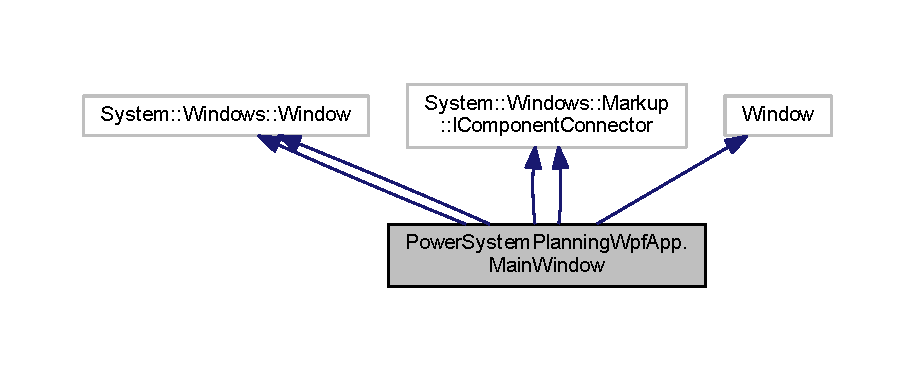
\includegraphics[width=350pt]{class_power_system_planning_wpf_app_1_1_main_window__inherit__graph}
\end{center}
\end{figure}


Collaboration diagram for Power\+System\+Planning\+Wpf\+App.\+Main\+Window\+:
\nopagebreak
\begin{figure}[H]
\begin{center}
\leavevmode
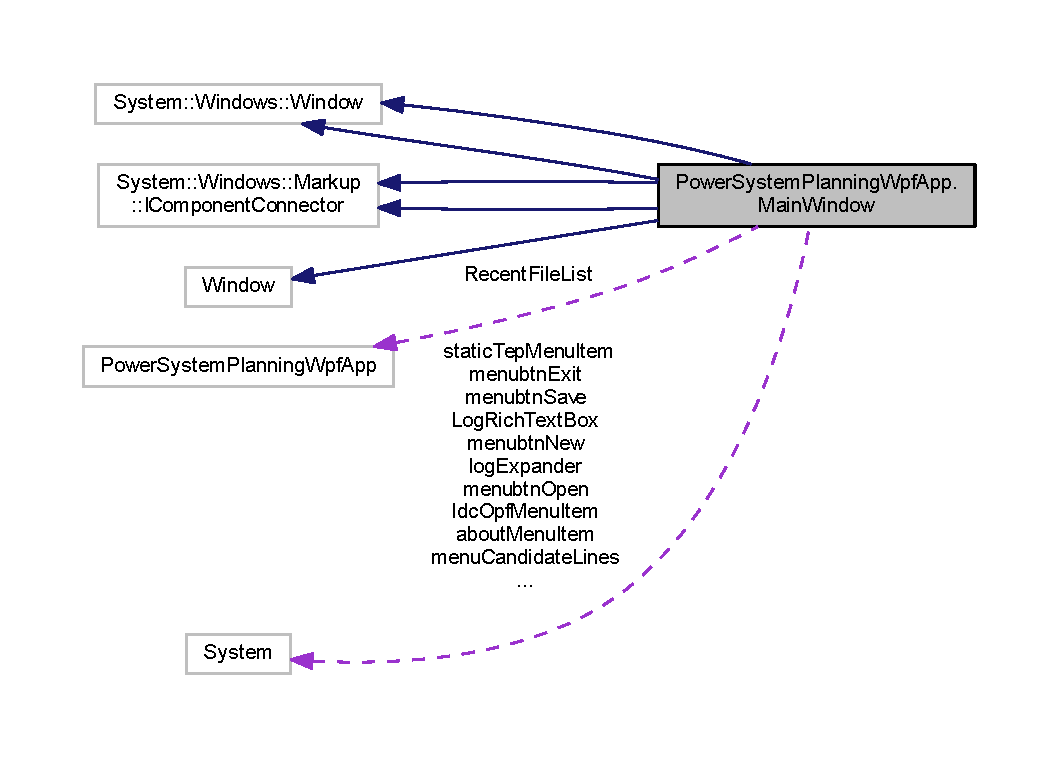
\includegraphics[width=350pt]{class_power_system_planning_wpf_app_1_1_main_window__coll__graph}
\end{center}
\end{figure}
\subsection*{Public Member Functions}
\begin{DoxyCompactItemize}
\item 
void \hyperlink{class_power_system_planning_wpf_app_1_1_main_window_aea9c6ec3e30669721d311bdb1fb964d8}{Initialize\+Component} ()
\begin{DoxyCompactList}\small\item\em Initialize\+Component \end{DoxyCompactList}\item 
void \hyperlink{class_power_system_planning_wpf_app_1_1_main_window_aea9c6ec3e30669721d311bdb1fb964d8}{Initialize\+Component} ()
\begin{DoxyCompactList}\small\item\em Initialize\+Component \end{DoxyCompactList}\end{DoxyCompactItemize}


\subsection{Detailed Description}
Interaction logic for Main\+Window.\+xaml 

\hyperlink{class_power_system_planning_wpf_app_1_1_main_window}{Main\+Window} 

\subsection{Member Function Documentation}
\index{Power\+System\+Planning\+Wpf\+App\+::\+Main\+Window@{Power\+System\+Planning\+Wpf\+App\+::\+Main\+Window}!Initialize\+Component@{Initialize\+Component}}
\index{Initialize\+Component@{Initialize\+Component}!Power\+System\+Planning\+Wpf\+App\+::\+Main\+Window@{Power\+System\+Planning\+Wpf\+App\+::\+Main\+Window}}
\subsubsection[{\texorpdfstring{Initialize\+Component()}{InitializeComponent()}}]{\setlength{\rightskip}{0pt plus 5cm}void Power\+System\+Planning\+Wpf\+App.\+Main\+Window.\+Initialize\+Component (
\begin{DoxyParamCaption}
{}
\end{DoxyParamCaption}
)\hspace{0.3cm}{\ttfamily [inline]}}\hypertarget{class_power_system_planning_wpf_app_1_1_main_window_aea9c6ec3e30669721d311bdb1fb964d8}{}\label{class_power_system_planning_wpf_app_1_1_main_window_aea9c6ec3e30669721d311bdb1fb964d8}


Initialize\+Component 

\index{Power\+System\+Planning\+Wpf\+App\+::\+Main\+Window@{Power\+System\+Planning\+Wpf\+App\+::\+Main\+Window}!Initialize\+Component@{Initialize\+Component}}
\index{Initialize\+Component@{Initialize\+Component}!Power\+System\+Planning\+Wpf\+App\+::\+Main\+Window@{Power\+System\+Planning\+Wpf\+App\+::\+Main\+Window}}
\subsubsection[{\texorpdfstring{Initialize\+Component()}{InitializeComponent()}}]{\setlength{\rightskip}{0pt plus 5cm}void Power\+System\+Planning\+Wpf\+App.\+Main\+Window.\+Initialize\+Component (
\begin{DoxyParamCaption}
{}
\end{DoxyParamCaption}
)\hspace{0.3cm}{\ttfamily [inline]}}\hypertarget{class_power_system_planning_wpf_app_1_1_main_window_aea9c6ec3e30669721d311bdb1fb964d8}{}\label{class_power_system_planning_wpf_app_1_1_main_window_aea9c6ec3e30669721d311bdb1fb964d8}


Initialize\+Component 



The documentation for this class was generated from the following files\+:\begin{DoxyCompactItemize}
\item 
Main\+Window.\+xaml.\+cs\item 
obj/\+Debug/Main\+Window.\+g.\+cs\item 
obj/\+Debug/Main\+Window.\+g.\+i.\+cs\end{DoxyCompactItemize}

\hypertarget{class_power_system_planning_wpf_app_1_1_control_utils_1_1_recent_file_list_1_1_menu_click_event_args}{}\section{Power\+System\+Planning\+Wpf\+App.\+Control\+Utils.\+Recent\+File\+List.\+Menu\+Click\+Event\+Args Class Reference}
\label{class_power_system_planning_wpf_app_1_1_control_utils_1_1_recent_file_list_1_1_menu_click_event_args}\index{Power\+System\+Planning\+Wpf\+App.\+Control\+Utils.\+Recent\+File\+List.\+Menu\+Click\+Event\+Args@{Power\+System\+Planning\+Wpf\+App.\+Control\+Utils.\+Recent\+File\+List.\+Menu\+Click\+Event\+Args}}


Inheritance diagram for Power\+System\+Planning\+Wpf\+App.\+Control\+Utils.\+Recent\+File\+List.\+Menu\+Click\+Event\+Args\+:\nopagebreak
\begin{figure}[H]
\begin{center}
\leavevmode
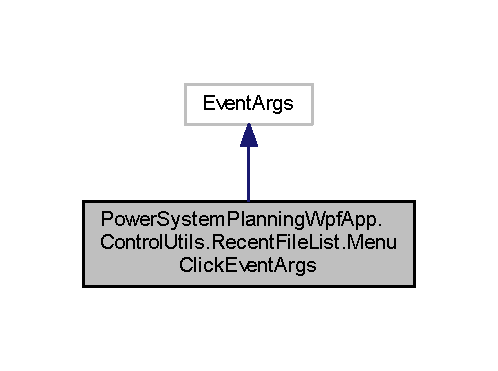
\includegraphics[width=239pt]{class_power_system_planning_wpf_app_1_1_control_utils_1_1_recent_file_list_1_1_menu_click_event_args__inherit__graph}
\end{center}
\end{figure}


Collaboration diagram for Power\+System\+Planning\+Wpf\+App.\+Control\+Utils.\+Recent\+File\+List.\+Menu\+Click\+Event\+Args\+:\nopagebreak
\begin{figure}[H]
\begin{center}
\leavevmode
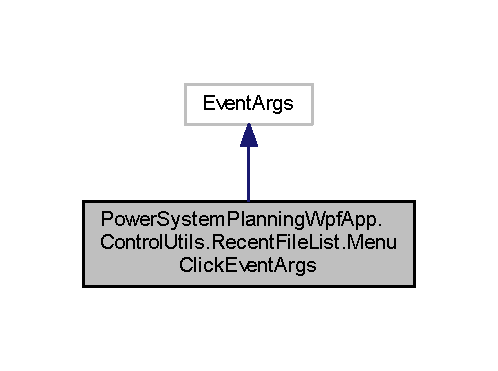
\includegraphics[width=239pt]{class_power_system_planning_wpf_app_1_1_control_utils_1_1_recent_file_list_1_1_menu_click_event_args__coll__graph}
\end{center}
\end{figure}
\subsection*{Public Member Functions}
\begin{DoxyCompactItemize}
\item 
{\bfseries Menu\+Click\+Event\+Args} (string filepath)\hypertarget{class_power_system_planning_wpf_app_1_1_control_utils_1_1_recent_file_list_1_1_menu_click_event_args_a4b59a33fb4c05bb796ebe23cf50e1695}{}\label{class_power_system_planning_wpf_app_1_1_control_utils_1_1_recent_file_list_1_1_menu_click_event_args_a4b59a33fb4c05bb796ebe23cf50e1695}

\end{DoxyCompactItemize}
\subsection*{Properties}
\begin{DoxyCompactItemize}
\item 
string {\bfseries Filepath}\hspace{0.3cm}{\ttfamily  \mbox{[}get\mbox{]}}\hypertarget{class_power_system_planning_wpf_app_1_1_control_utils_1_1_recent_file_list_1_1_menu_click_event_args_a5dd55be771936c2222924eda6e5bf465}{}\label{class_power_system_planning_wpf_app_1_1_control_utils_1_1_recent_file_list_1_1_menu_click_event_args_a5dd55be771936c2222924eda6e5bf465}

\end{DoxyCompactItemize}


The documentation for this class was generated from the following file\+:\begin{DoxyCompactItemize}
\item 
Control\+Utils/Recent\+File\+List.\+cs\end{DoxyCompactItemize}

\input{class_power_system_planning_wpf_app_1_1_l_d_c_1_1_o_p_f_l_d_c_results_control}
\input{class_power_system_planning_wpf_app_1_1_l_d_c_1_1_o_p_f_l_d_c_results_window}
\input{class_power_system_planning_wpf_app_1_1_o_p_f_1_1_o_p_f_results_control}
\input{class_power_system_planning_wpf_app_1_1_o_p_f_1_1_o_p_f_results_window}
\input{class_power_system_planning_wpf_app_1_1_o_p_f_1_1_o_p_f_run_window}
\input{class_power_system_planning_wpf_app_1_1_l_d_c_1_1_optimize_o_p_f_l_d_c}
\hypertarget{class_power_system_planning_wpf_app_1_1_control_utils_1_1_recent_file_list}{}\section{Power\+System\+Planning\+Wpf\+App.\+Control\+Utils.\+Recent\+File\+List Class Reference}
\label{class_power_system_planning_wpf_app_1_1_control_utils_1_1_recent_file_list}\index{Power\+System\+Planning\+Wpf\+App.\+Control\+Utils.\+Recent\+File\+List@{Power\+System\+Planning\+Wpf\+App.\+Control\+Utils.\+Recent\+File\+List}}


Inheritance diagram for Power\+System\+Planning\+Wpf\+App.\+Control\+Utils.\+Recent\+File\+List\+:\nopagebreak
\begin{figure}[H]
\begin{center}
\leavevmode
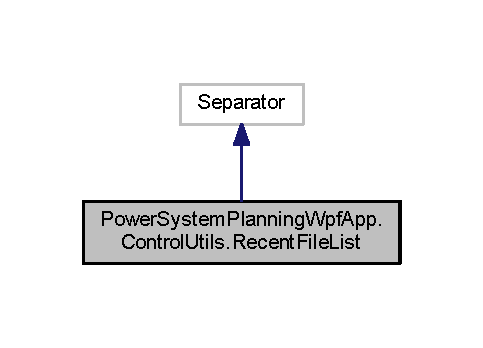
\includegraphics[width=232pt]{class_power_system_planning_wpf_app_1_1_control_utils_1_1_recent_file_list__inherit__graph}
\end{center}
\end{figure}


Collaboration diagram for Power\+System\+Planning\+Wpf\+App.\+Control\+Utils.\+Recent\+File\+List\+:\nopagebreak
\begin{figure}[H]
\begin{center}
\leavevmode
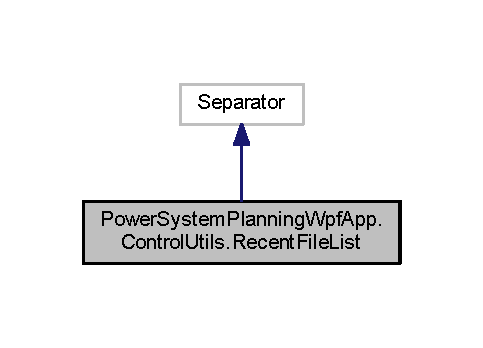
\includegraphics[width=232pt]{class_power_system_planning_wpf_app_1_1_control_utils_1_1_recent_file_list__coll__graph}
\end{center}
\end{figure}
\subsection*{Classes}
\begin{DoxyCompactItemize}
\item 
interface \hyperlink{interface_power_system_planning_wpf_app_1_1_control_utils_1_1_recent_file_list_1_1_i_persist}{I\+Persist}
\item 
class \hyperlink{class_power_system_planning_wpf_app_1_1_control_utils_1_1_recent_file_list_1_1_menu_click_event_args}{Menu\+Click\+Event\+Args}
\end{DoxyCompactItemize}
\subsection*{Public Member Functions}
\begin{DoxyCompactItemize}
\item 
void {\bfseries Use\+Registry\+Persister} ()\hypertarget{class_power_system_planning_wpf_app_1_1_control_utils_1_1_recent_file_list_a84700150f6c11115f006032130bdc22b}{}\label{class_power_system_planning_wpf_app_1_1_control_utils_1_1_recent_file_list_a84700150f6c11115f006032130bdc22b}

\item 
void {\bfseries Use\+Registry\+Persister} (string key)\hypertarget{class_power_system_planning_wpf_app_1_1_control_utils_1_1_recent_file_list_a1a2dc5674711f02f8cffddc047c23cd2}{}\label{class_power_system_planning_wpf_app_1_1_control_utils_1_1_recent_file_list_a1a2dc5674711f02f8cffddc047c23cd2}

\item 
void {\bfseries Use\+Xml\+Persister} ()\hypertarget{class_power_system_planning_wpf_app_1_1_control_utils_1_1_recent_file_list_a306d159c9e67841924fa726455c78c6d}{}\label{class_power_system_planning_wpf_app_1_1_control_utils_1_1_recent_file_list_a306d159c9e67841924fa726455c78c6d}

\item 
void {\bfseries Use\+Xml\+Persister} (string filepath)\hypertarget{class_power_system_planning_wpf_app_1_1_control_utils_1_1_recent_file_list_a81c0eb8e2f77e20d2b4dc4585c77a512}{}\label{class_power_system_planning_wpf_app_1_1_control_utils_1_1_recent_file_list_a81c0eb8e2f77e20d2b4dc4585c77a512}

\item 
void {\bfseries Use\+Xml\+Persister} (Stream stream)\hypertarget{class_power_system_planning_wpf_app_1_1_control_utils_1_1_recent_file_list_af51e5ee1dae68964628940a8c59d392e}{}\label{class_power_system_planning_wpf_app_1_1_control_utils_1_1_recent_file_list_af51e5ee1dae68964628940a8c59d392e}

\item 
delegate string {\bfseries Get\+Menu\+Item\+Text\+Delegate} (int index, string filepath)\hypertarget{class_power_system_planning_wpf_app_1_1_control_utils_1_1_recent_file_list_a4c265c426fe8be2c22ca7dba76a17289}{}\label{class_power_system_planning_wpf_app_1_1_control_utils_1_1_recent_file_list_a4c265c426fe8be2c22ca7dba76a17289}

\item 
void {\bfseries Remove\+File} (string filepath)\hypertarget{class_power_system_planning_wpf_app_1_1_control_utils_1_1_recent_file_list_a1cb48459a0901d95d4fd16c9e44b0e17}{}\label{class_power_system_planning_wpf_app_1_1_control_utils_1_1_recent_file_list_a1cb48459a0901d95d4fd16c9e44b0e17}

\item 
void {\bfseries Insert\+File} (string filepath)\hypertarget{class_power_system_planning_wpf_app_1_1_control_utils_1_1_recent_file_list_a03a6cf8a832adcf8613bccbf31f47089}{}\label{class_power_system_planning_wpf_app_1_1_control_utils_1_1_recent_file_list_a03a6cf8a832adcf8613bccbf31f47089}

\end{DoxyCompactItemize}
\subsection*{Static Public Member Functions}
\begin{DoxyCompactItemize}
\item 
static string \hyperlink{class_power_system_planning_wpf_app_1_1_control_utils_1_1_recent_file_list_a98ebf9d14956e17f7973efde04d5281b}{Shorten\+Pathname} (string pathname, int max\+Length)
\begin{DoxyCompactList}\small\item\em Shortens a pathname for display purposes. \end{DoxyCompactList}\end{DoxyCompactItemize}
\subsection*{Protected Member Functions}
\begin{DoxyCompactItemize}
\item 
virtual void {\bfseries On\+Menu\+Click} (Menu\+Item menu\+Item)\hypertarget{class_power_system_planning_wpf_app_1_1_control_utils_1_1_recent_file_list_aa49aa79c00c1fed4603b820e7fa4d429}{}\label{class_power_system_planning_wpf_app_1_1_control_utils_1_1_recent_file_list_aa49aa79c00c1fed4603b820e7fa4d429}

\end{DoxyCompactItemize}
\subsection*{Properties}
\begin{DoxyCompactItemize}
\item 
\hyperlink{interface_power_system_planning_wpf_app_1_1_control_utils_1_1_recent_file_list_1_1_i_persist}{I\+Persist} {\bfseries Persister}\hspace{0.3cm}{\ttfamily  \mbox{[}get, set\mbox{]}}\hypertarget{class_power_system_planning_wpf_app_1_1_control_utils_1_1_recent_file_list_a858f94dc2ebc154982ac5769574400bf}{}\label{class_power_system_planning_wpf_app_1_1_control_utils_1_1_recent_file_list_a858f94dc2ebc154982ac5769574400bf}

\item 
int {\bfseries Max\+Number\+Of\+Files}\hspace{0.3cm}{\ttfamily  \mbox{[}get, set\mbox{]}}\hypertarget{class_power_system_planning_wpf_app_1_1_control_utils_1_1_recent_file_list_af2df62a154d5c554bc1695eb469a0f31}{}\label{class_power_system_planning_wpf_app_1_1_control_utils_1_1_recent_file_list_af2df62a154d5c554bc1695eb469a0f31}

\item 
int {\bfseries Max\+Path\+Length}\hspace{0.3cm}{\ttfamily  \mbox{[}get, set\mbox{]}}\hypertarget{class_power_system_planning_wpf_app_1_1_control_utils_1_1_recent_file_list_ad9a93bd797b563618155bc58d4169c85}{}\label{class_power_system_planning_wpf_app_1_1_control_utils_1_1_recent_file_list_ad9a93bd797b563618155bc58d4169c85}

\item 
Menu\+Item {\bfseries File\+Menu}\hspace{0.3cm}{\ttfamily  \mbox{[}get\mbox{]}}\hypertarget{class_power_system_planning_wpf_app_1_1_control_utils_1_1_recent_file_list_a8eb18ef52d6a7491ce995f8a5becf0fd}{}\label{class_power_system_planning_wpf_app_1_1_control_utils_1_1_recent_file_list_a8eb18ef52d6a7491ce995f8a5becf0fd}

\item 
string \hyperlink{class_power_system_planning_wpf_app_1_1_control_utils_1_1_recent_file_list_aae95e2ccda33122a193e35af9bf6aa0e}{Menu\+Item\+Format\+One\+To\+Nine}\hspace{0.3cm}{\ttfamily  \mbox{[}get, set\mbox{]}}
\begin{DoxyCompactList}\small\item\em Used in\+: String.\+Format( Menu\+Item\+Format, index, filepath, display\+Path ); Default = \char`\"{}\+\_\+\{0\}\+:  \{2\}\char`\"{} \end{DoxyCompactList}\item 
string \hyperlink{class_power_system_planning_wpf_app_1_1_control_utils_1_1_recent_file_list_a27d7ee892ff4ad876fcee4e8b6f7c076}{Menu\+Item\+Format\+Ten\+Plus}\hspace{0.3cm}{\ttfamily  \mbox{[}get, set\mbox{]}}
\begin{DoxyCompactList}\small\item\em Used in\+: String.\+Format( Menu\+Item\+Format, index, filepath, display\+Path ); Default = \char`\"{}\{0\}\+:  \{2\}\char`\"{} \end{DoxyCompactList}\item 
Get\+Menu\+Item\+Text\+Delegate {\bfseries Get\+Menu\+Item\+Text\+Handler}\hspace{0.3cm}{\ttfamily  \mbox{[}get, set\mbox{]}}\hypertarget{class_power_system_planning_wpf_app_1_1_control_utils_1_1_recent_file_list_a0541e623b6977a2672c5a6e54d8af2b4}{}\label{class_power_system_planning_wpf_app_1_1_control_utils_1_1_recent_file_list_a0541e623b6977a2672c5a6e54d8af2b4}

\item 
List$<$ string $>$ {\bfseries Recent\+Files}\hspace{0.3cm}{\ttfamily  \mbox{[}get\mbox{]}}\hypertarget{class_power_system_planning_wpf_app_1_1_control_utils_1_1_recent_file_list_ab646cd45024c3a96574b90db7114e23a}{}\label{class_power_system_planning_wpf_app_1_1_control_utils_1_1_recent_file_list_ab646cd45024c3a96574b90db7114e23a}

\end{DoxyCompactItemize}
\subsection*{Events}
\begin{DoxyCompactItemize}
\item 
Event\+Handler$<$ \hyperlink{class_power_system_planning_wpf_app_1_1_control_utils_1_1_recent_file_list_1_1_menu_click_event_args}{Menu\+Click\+Event\+Args} $>$ {\bfseries Menu\+Click}\hypertarget{class_power_system_planning_wpf_app_1_1_control_utils_1_1_recent_file_list_ad5108b19820ca3c4d54534f739b36ade}{}\label{class_power_system_planning_wpf_app_1_1_control_utils_1_1_recent_file_list_ad5108b19820ca3c4d54534f739b36ade}

\end{DoxyCompactItemize}


\subsection{Member Function Documentation}
\index{Power\+System\+Planning\+Wpf\+App\+::\+Control\+Utils\+::\+Recent\+File\+List@{Power\+System\+Planning\+Wpf\+App\+::\+Control\+Utils\+::\+Recent\+File\+List}!Shorten\+Pathname@{Shorten\+Pathname}}
\index{Shorten\+Pathname@{Shorten\+Pathname}!Power\+System\+Planning\+Wpf\+App\+::\+Control\+Utils\+::\+Recent\+File\+List@{Power\+System\+Planning\+Wpf\+App\+::\+Control\+Utils\+::\+Recent\+File\+List}}
\subsubsection[{\texorpdfstring{Shorten\+Pathname(string pathname, int max\+Length)}{ShortenPathname(string pathname, int maxLength)}}]{\setlength{\rightskip}{0pt plus 5cm}static string Power\+System\+Planning\+Wpf\+App.\+Control\+Utils.\+Recent\+File\+List.\+Shorten\+Pathname (
\begin{DoxyParamCaption}
\item[{string}]{pathname, }
\item[{int}]{max\+Length}
\end{DoxyParamCaption}
)\hspace{0.3cm}{\ttfamily [inline]}, {\ttfamily [static]}}\hypertarget{class_power_system_planning_wpf_app_1_1_control_utils_1_1_recent_file_list_a98ebf9d14956e17f7973efde04d5281b}{}\label{class_power_system_planning_wpf_app_1_1_control_utils_1_1_recent_file_list_a98ebf9d14956e17f7973efde04d5281b}


Shortens a pathname for display purposes. 

The pathname to shorten.

The maximum number of characters to be displayed.

Shortens a pathname by either removing consecutive components of a path and/or by removing characters from the end of the filename and replacing then with three elipses (...) 

In all cases, the root of the passed path will be preserved in it\textquotesingle{}s entirety.

If a U\+NC path is used or the pathname and max\+Length are particularly short, the resulting path may be longer than max\+Length.

This method expects fully resolved pathnames to be passed to it. (Use Path.\+Get\+Full\+Path() to obtain this.)

\begin{DoxyReturn}{Returns}

\end{DoxyReturn}


\subsection{Property Documentation}
\index{Power\+System\+Planning\+Wpf\+App\+::\+Control\+Utils\+::\+Recent\+File\+List@{Power\+System\+Planning\+Wpf\+App\+::\+Control\+Utils\+::\+Recent\+File\+List}!Menu\+Item\+Format\+One\+To\+Nine@{Menu\+Item\+Format\+One\+To\+Nine}}
\index{Menu\+Item\+Format\+One\+To\+Nine@{Menu\+Item\+Format\+One\+To\+Nine}!Power\+System\+Planning\+Wpf\+App\+::\+Control\+Utils\+::\+Recent\+File\+List@{Power\+System\+Planning\+Wpf\+App\+::\+Control\+Utils\+::\+Recent\+File\+List}}
\subsubsection[{\texorpdfstring{Menu\+Item\+Format\+One\+To\+Nine}{MenuItemFormatOneToNine}}]{\setlength{\rightskip}{0pt plus 5cm}string Power\+System\+Planning\+Wpf\+App.\+Control\+Utils.\+Recent\+File\+List.\+Menu\+Item\+Format\+One\+To\+Nine\hspace{0.3cm}{\ttfamily [get]}, {\ttfamily [set]}}\hypertarget{class_power_system_planning_wpf_app_1_1_control_utils_1_1_recent_file_list_aae95e2ccda33122a193e35af9bf6aa0e}{}\label{class_power_system_planning_wpf_app_1_1_control_utils_1_1_recent_file_list_aae95e2ccda33122a193e35af9bf6aa0e}


Used in\+: String.\+Format( Menu\+Item\+Format, index, filepath, display\+Path ); Default = \char`\"{}\+\_\+\{0\}\+:  \{2\}\char`\"{} 

\index{Power\+System\+Planning\+Wpf\+App\+::\+Control\+Utils\+::\+Recent\+File\+List@{Power\+System\+Planning\+Wpf\+App\+::\+Control\+Utils\+::\+Recent\+File\+List}!Menu\+Item\+Format\+Ten\+Plus@{Menu\+Item\+Format\+Ten\+Plus}}
\index{Menu\+Item\+Format\+Ten\+Plus@{Menu\+Item\+Format\+Ten\+Plus}!Power\+System\+Planning\+Wpf\+App\+::\+Control\+Utils\+::\+Recent\+File\+List@{Power\+System\+Planning\+Wpf\+App\+::\+Control\+Utils\+::\+Recent\+File\+List}}
\subsubsection[{\texorpdfstring{Menu\+Item\+Format\+Ten\+Plus}{MenuItemFormatTenPlus}}]{\setlength{\rightskip}{0pt plus 5cm}string Power\+System\+Planning\+Wpf\+App.\+Control\+Utils.\+Recent\+File\+List.\+Menu\+Item\+Format\+Ten\+Plus\hspace{0.3cm}{\ttfamily [get]}, {\ttfamily [set]}}\hypertarget{class_power_system_planning_wpf_app_1_1_control_utils_1_1_recent_file_list_a27d7ee892ff4ad876fcee4e8b6f7c076}{}\label{class_power_system_planning_wpf_app_1_1_control_utils_1_1_recent_file_list_a27d7ee892ff4ad876fcee4e8b6f7c076}


Used in\+: String.\+Format( Menu\+Item\+Format, index, filepath, display\+Path ); Default = \char`\"{}\{0\}\+:  \{2\}\char`\"{} 



The documentation for this class was generated from the following file\+:\begin{DoxyCompactItemize}
\item 
Control\+Utils/Recent\+File\+List.\+cs\end{DoxyCompactItemize}

\hypertarget{class_power_system_planning_wpf_app_1_1_o_p_f_1_1_run_economic_dispatch}{}\section{Power\+System\+Planning\+Wpf\+App.\+O\+P\+F.\+Run\+Economic\+Dispatch Class Reference}
\label{class_power_system_planning_wpf_app_1_1_o_p_f_1_1_run_economic_dispatch}\index{Power\+System\+Planning\+Wpf\+App.\+O\+P\+F.\+Run\+Economic\+Dispatch@{Power\+System\+Planning\+Wpf\+App.\+O\+P\+F.\+Run\+Economic\+Dispatch}}


\hyperlink{class_power_system_planning_wpf_app_1_1_o_p_f_1_1_run_economic_dispatch}{Run\+Economic\+Dispatch}  




Inheritance diagram for Power\+System\+Planning\+Wpf\+App.\+O\+P\+F.\+Run\+Economic\+Dispatch\+:\nopagebreak
\begin{figure}[H]
\begin{center}
\leavevmode
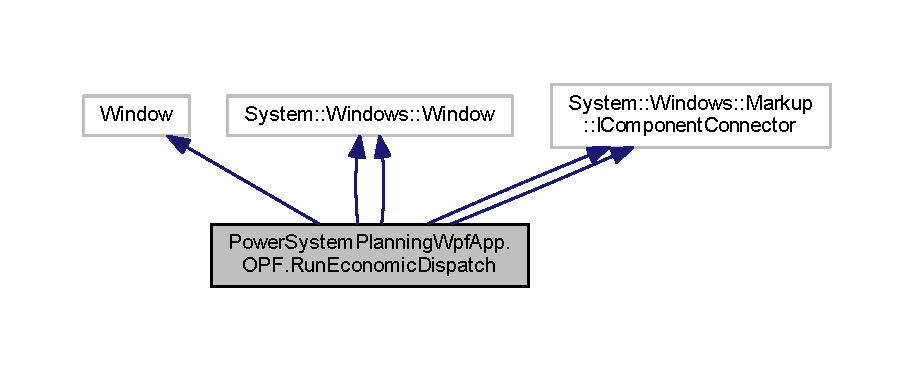
\includegraphics[width=350pt]{class_power_system_planning_wpf_app_1_1_o_p_f_1_1_run_economic_dispatch__inherit__graph}
\end{center}
\end{figure}


Collaboration diagram for Power\+System\+Planning\+Wpf\+App.\+O\+P\+F.\+Run\+Economic\+Dispatch\+:\nopagebreak
\begin{figure}[H]
\begin{center}
\leavevmode
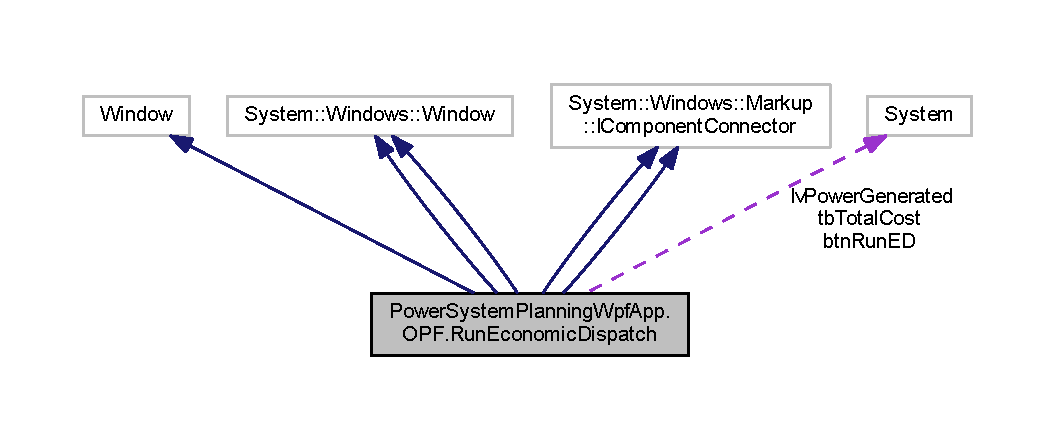
\includegraphics[width=350pt]{class_power_system_planning_wpf_app_1_1_o_p_f_1_1_run_economic_dispatch__coll__graph}
\end{center}
\end{figure}
\subsection*{Public Member Functions}
\begin{DoxyCompactItemize}
\item 
void \hyperlink{class_power_system_planning_wpf_app_1_1_o_p_f_1_1_run_economic_dispatch_adb304aa76ae18ccc2e1b962a69e7f317}{Initialize\+Component} ()
\begin{DoxyCompactList}\small\item\em Initialize\+Component \end{DoxyCompactList}\end{DoxyCompactItemize}


\subsection{Detailed Description}
\hyperlink{class_power_system_planning_wpf_app_1_1_o_p_f_1_1_run_economic_dispatch}{Run\+Economic\+Dispatch} 



\subsection{Member Function Documentation}
\index{Power\+System\+Planning\+Wpf\+App\+::\+O\+P\+F\+::\+Run\+Economic\+Dispatch@{Power\+System\+Planning\+Wpf\+App\+::\+O\+P\+F\+::\+Run\+Economic\+Dispatch}!Initialize\+Component@{Initialize\+Component}}
\index{Initialize\+Component@{Initialize\+Component}!Power\+System\+Planning\+Wpf\+App\+::\+O\+P\+F\+::\+Run\+Economic\+Dispatch@{Power\+System\+Planning\+Wpf\+App\+::\+O\+P\+F\+::\+Run\+Economic\+Dispatch}}
\subsubsection[{\texorpdfstring{Initialize\+Component()}{InitializeComponent()}}]{\setlength{\rightskip}{0pt plus 5cm}void Power\+System\+Planning\+Wpf\+App.\+O\+P\+F.\+Run\+Economic\+Dispatch.\+Initialize\+Component (
\begin{DoxyParamCaption}
{}
\end{DoxyParamCaption}
)\hspace{0.3cm}{\ttfamily [inline]}}\hypertarget{class_power_system_planning_wpf_app_1_1_o_p_f_1_1_run_economic_dispatch_adb304aa76ae18ccc2e1b962a69e7f317}{}\label{class_power_system_planning_wpf_app_1_1_o_p_f_1_1_run_economic_dispatch_adb304aa76ae18ccc2e1b962a69e7f317}


Initialize\+Component 



The documentation for this class was generated from the following file\+:\begin{DoxyCompactItemize}
\item 
obj/\+Debug/\+O\+P\+F/Run\+Economic\+Dispatch.\+g.\+i.\+cs\end{DoxyCompactItemize}

\input{class_power_system_planning_wpf_app_1_1_l_d_c_1_1_run_l_d_c}
\hypertarget{class_power_system_planning_wpf_app_1_1_o_p_f_1_1_run_o_p_f_window}{}\section{Power\+System\+Planning\+Wpf\+App.\+O\+P\+F.\+Run\+O\+P\+F\+Window Class Reference}
\label{class_power_system_planning_wpf_app_1_1_o_p_f_1_1_run_o_p_f_window}\index{Power\+System\+Planning\+Wpf\+App.\+O\+P\+F.\+Run\+O\+P\+F\+Window@{Power\+System\+Planning\+Wpf\+App.\+O\+P\+F.\+Run\+O\+P\+F\+Window}}


\hyperlink{class_power_system_planning_wpf_app_1_1_o_p_f_1_1_run_o_p_f_window}{Run\+O\+P\+F\+Window}  




Inheritance diagram for Power\+System\+Planning\+Wpf\+App.\+O\+P\+F.\+Run\+O\+P\+F\+Window\+:\nopagebreak
\begin{figure}[H]
\begin{center}
\leavevmode
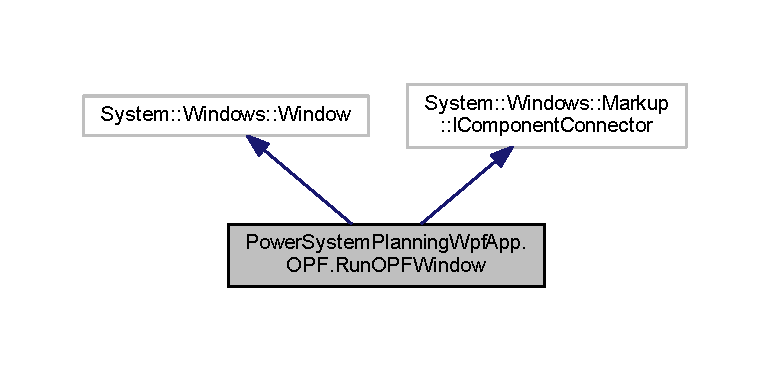
\includegraphics[width=350pt]{class_power_system_planning_wpf_app_1_1_o_p_f_1_1_run_o_p_f_window__inherit__graph}
\end{center}
\end{figure}


Collaboration diagram for Power\+System\+Planning\+Wpf\+App.\+O\+P\+F.\+Run\+O\+P\+F\+Window\+:\nopagebreak
\begin{figure}[H]
\begin{center}
\leavevmode
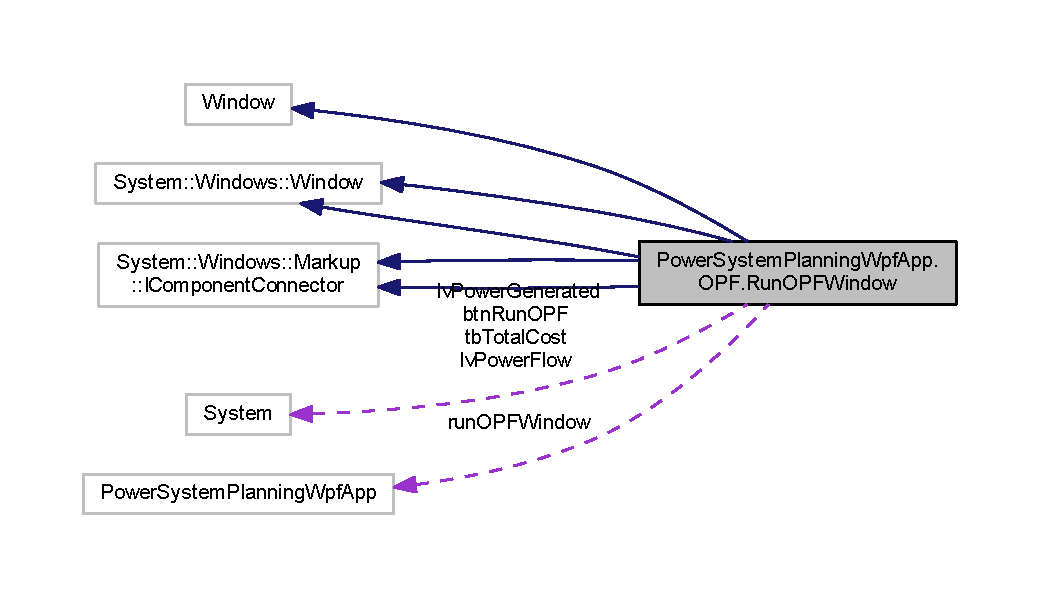
\includegraphics[width=350pt]{class_power_system_planning_wpf_app_1_1_o_p_f_1_1_run_o_p_f_window__coll__graph}
\end{center}
\end{figure}
\subsection*{Public Member Functions}
\begin{DoxyCompactItemize}
\item 
void \hyperlink{class_power_system_planning_wpf_app_1_1_o_p_f_1_1_run_o_p_f_window_a91ab91e324339cf90a9f3265e2b3e636}{Initialize\+Component} ()
\begin{DoxyCompactList}\small\item\em Initialize\+Component \end{DoxyCompactList}\item 
void \hyperlink{class_power_system_planning_wpf_app_1_1_o_p_f_1_1_run_o_p_f_window_a91ab91e324339cf90a9f3265e2b3e636}{Initialize\+Component} ()
\begin{DoxyCompactList}\small\item\em Initialize\+Component \end{DoxyCompactList}\item 
{\bfseries Run\+O\+P\+F\+Window} (Power\+System power\+System)\hypertarget{class_power_system_planning_wpf_app_1_1_o_p_f_1_1_run_o_p_f_window_afc3cbde00426a5913ef9996a89a553e4}{}\label{class_power_system_planning_wpf_app_1_1_o_p_f_1_1_run_o_p_f_window_afc3cbde00426a5913ef9996a89a553e4}

\end{DoxyCompactItemize}


\subsection{Detailed Description}
\hyperlink{class_power_system_planning_wpf_app_1_1_o_p_f_1_1_run_o_p_f_window}{Run\+O\+P\+F\+Window} 

Interaction logic for Run\+O\+P\+F\+Window.\+xaml 

\subsection{Member Function Documentation}
\index{Power\+System\+Planning\+Wpf\+App\+::\+O\+P\+F\+::\+Run\+O\+P\+F\+Window@{Power\+System\+Planning\+Wpf\+App\+::\+O\+P\+F\+::\+Run\+O\+P\+F\+Window}!Initialize\+Component@{Initialize\+Component}}
\index{Initialize\+Component@{Initialize\+Component}!Power\+System\+Planning\+Wpf\+App\+::\+O\+P\+F\+::\+Run\+O\+P\+F\+Window@{Power\+System\+Planning\+Wpf\+App\+::\+O\+P\+F\+::\+Run\+O\+P\+F\+Window}}
\subsubsection[{\texorpdfstring{Initialize\+Component()}{InitializeComponent()}}]{\setlength{\rightskip}{0pt plus 5cm}void Power\+System\+Planning\+Wpf\+App.\+O\+P\+F.\+Run\+O\+P\+F\+Window.\+Initialize\+Component (
\begin{DoxyParamCaption}
{}
\end{DoxyParamCaption}
)\hspace{0.3cm}{\ttfamily [inline]}}\hypertarget{class_power_system_planning_wpf_app_1_1_o_p_f_1_1_run_o_p_f_window_a91ab91e324339cf90a9f3265e2b3e636}{}\label{class_power_system_planning_wpf_app_1_1_o_p_f_1_1_run_o_p_f_window_a91ab91e324339cf90a9f3265e2b3e636}


Initialize\+Component 

\index{Power\+System\+Planning\+Wpf\+App\+::\+O\+P\+F\+::\+Run\+O\+P\+F\+Window@{Power\+System\+Planning\+Wpf\+App\+::\+O\+P\+F\+::\+Run\+O\+P\+F\+Window}!Initialize\+Component@{Initialize\+Component}}
\index{Initialize\+Component@{Initialize\+Component}!Power\+System\+Planning\+Wpf\+App\+::\+O\+P\+F\+::\+Run\+O\+P\+F\+Window@{Power\+System\+Planning\+Wpf\+App\+::\+O\+P\+F\+::\+Run\+O\+P\+F\+Window}}
\subsubsection[{\texorpdfstring{Initialize\+Component()}{InitializeComponent()}}]{\setlength{\rightskip}{0pt plus 5cm}void Power\+System\+Planning\+Wpf\+App.\+O\+P\+F.\+Run\+O\+P\+F\+Window.\+Initialize\+Component (
\begin{DoxyParamCaption}
{}
\end{DoxyParamCaption}
)\hspace{0.3cm}{\ttfamily [inline]}}\hypertarget{class_power_system_planning_wpf_app_1_1_o_p_f_1_1_run_o_p_f_window_a91ab91e324339cf90a9f3265e2b3e636}{}\label{class_power_system_planning_wpf_app_1_1_o_p_f_1_1_run_o_p_f_window_a91ab91e324339cf90a9f3265e2b3e636}


Initialize\+Component 



The documentation for this class was generated from the following files\+:\begin{DoxyCompactItemize}
\item 
obj/\+Debug/\+O\+P\+F/Run\+O\+P\+F\+Window.\+g.\+cs\item 
obj/\+Debug/\+O\+P\+F/Run\+O\+P\+F\+Window.\+g.\+i.\+cs\item 
O\+P\+F/Run\+O\+P\+F\+Window.\+xaml.\+cs\end{DoxyCompactItemize}

\input{class_power_system_planning_wpf_app_1_1_scenario_t_e_p_1_1_scenario_t_e_p_window}
\hypertarget{class_power_system_planning_wpf_app_1_1_control_utils_1_1_simple_backend_model}{}\section{Power\+System\+Planning\+Wpf\+App.\+Control\+Utils.\+Simple\+Backend\+Model Class Reference}
\label{class_power_system_planning_wpf_app_1_1_control_utils_1_1_simple_backend_model}\index{Power\+System\+Planning\+Wpf\+App.\+Control\+Utils.\+Simple\+Backend\+Model@{Power\+System\+Planning\+Wpf\+App.\+Control\+Utils.\+Simple\+Backend\+Model}}
\subsection*{Public Attributes}
\begin{DoxyCompactItemize}
\item 
Binding\+List$<$ \hyperlink{class_power_system_planning_wpf_app_1_1_control_utils_1_1_simple_backend_object}{Simple\+Backend\+Object} $>$ {\bfseries backendlist}\hypertarget{class_power_system_planning_wpf_app_1_1_control_utils_1_1_simple_backend_model_a69a6c81750e3c4af0ea2a399592499c6}{}\label{class_power_system_planning_wpf_app_1_1_control_utils_1_1_simple_backend_model_a69a6c81750e3c4af0ea2a399592499c6}

\end{DoxyCompactItemize}


The documentation for this class was generated from the following file\+:\begin{DoxyCompactItemize}
\item 
Control\+Utils/Window\+Datagrid\+Test.\+xaml.\+cs\end{DoxyCompactItemize}

\hypertarget{class_power_system_planning_wpf_app_1_1_control_utils_1_1_simple_backend_object}{}\section{Power\+System\+Planning\+Wpf\+App.\+Control\+Utils.\+Simple\+Backend\+Object Class Reference}
\label{class_power_system_planning_wpf_app_1_1_control_utils_1_1_simple_backend_object}\index{Power\+System\+Planning\+Wpf\+App.\+Control\+Utils.\+Simple\+Backend\+Object@{Power\+System\+Planning\+Wpf\+App.\+Control\+Utils.\+Simple\+Backend\+Object}}


Inheritance diagram for Power\+System\+Planning\+Wpf\+App.\+Control\+Utils.\+Simple\+Backend\+Object\+:\nopagebreak
\begin{figure}[H]
\begin{center}
\leavevmode
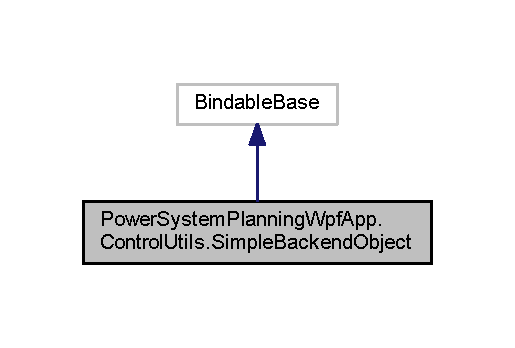
\includegraphics[width=247pt]{class_power_system_planning_wpf_app_1_1_control_utils_1_1_simple_backend_object__inherit__graph}
\end{center}
\end{figure}


Collaboration diagram for Power\+System\+Planning\+Wpf\+App.\+Control\+Utils.\+Simple\+Backend\+Object\+:\nopagebreak
\begin{figure}[H]
\begin{center}
\leavevmode
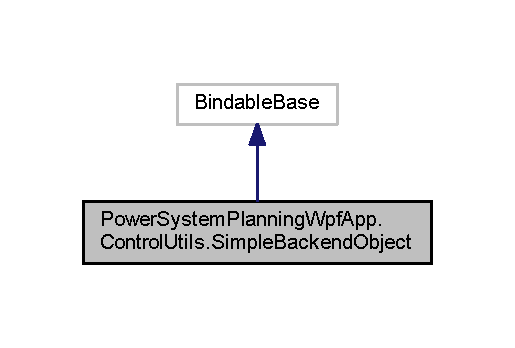
\includegraphics[width=247pt]{class_power_system_planning_wpf_app_1_1_control_utils_1_1_simple_backend_object__coll__graph}
\end{center}
\end{figure}
\subsection*{Public Member Functions}
\begin{DoxyCompactItemize}
\item 
{\bfseries Simple\+Backend\+Object} (string name, int age)\hypertarget{class_power_system_planning_wpf_app_1_1_control_utils_1_1_simple_backend_object_af99b564ac0c1e4f67fc8c0d045e3a68c}{}\label{class_power_system_planning_wpf_app_1_1_control_utils_1_1_simple_backend_object_af99b564ac0c1e4f67fc8c0d045e3a68c}

\end{DoxyCompactItemize}
\subsection*{Properties}
\begin{DoxyCompactItemize}
\item 
string {\bfseries Name}\hspace{0.3cm}{\ttfamily  \mbox{[}get, set\mbox{]}}\hypertarget{class_power_system_planning_wpf_app_1_1_control_utils_1_1_simple_backend_object_a43680268921f04aa8c406c2b7f0523eb}{}\label{class_power_system_planning_wpf_app_1_1_control_utils_1_1_simple_backend_object_a43680268921f04aa8c406c2b7f0523eb}

\item 
int {\bfseries Age}\hspace{0.3cm}{\ttfamily  \mbox{[}get, set\mbox{]}}\hypertarget{class_power_system_planning_wpf_app_1_1_control_utils_1_1_simple_backend_object_ab43f860f6996a28d5f7ea99d04006bba}{}\label{class_power_system_planning_wpf_app_1_1_control_utils_1_1_simple_backend_object_ab43f860f6996a28d5f7ea99d04006bba}

\end{DoxyCompactItemize}


The documentation for this class was generated from the following file\+:\begin{DoxyCompactItemize}
\item 
Control\+Utils/Window\+Datagrid\+Test.\+xaml.\+cs\end{DoxyCompactItemize}

\hypertarget{class_power_system_planning_wpf_app_1_1_control_utils_1_1_simple_terminal}{}\section{Power\+System\+Planning\+Wpf\+App.\+Control\+Utils.\+Simple\+Terminal Class Reference}
\label{class_power_system_planning_wpf_app_1_1_control_utils_1_1_simple_terminal}\index{Power\+System\+Planning\+Wpf\+App.\+Control\+Utils.\+Simple\+Terminal@{Power\+System\+Planning\+Wpf\+App.\+Control\+Utils.\+Simple\+Terminal}}


Interaction logic for Simple\+Terminal.\+xaml  




Inheritance diagram for Power\+System\+Planning\+Wpf\+App.\+Control\+Utils.\+Simple\+Terminal\+:\nopagebreak
\begin{figure}[H]
\begin{center}
\leavevmode
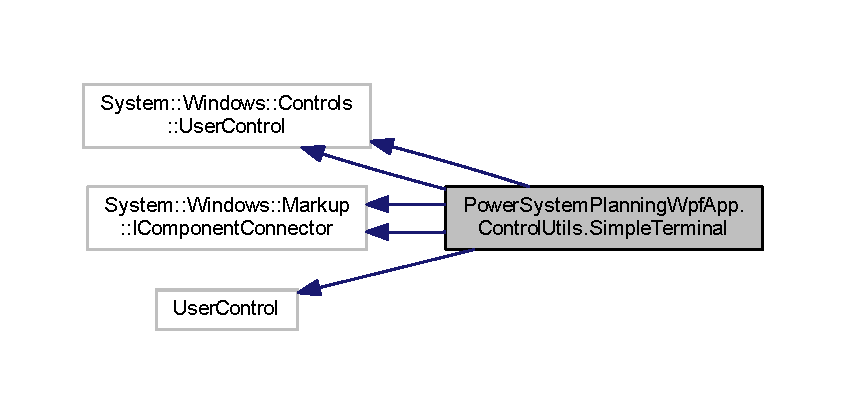
\includegraphics[width=350pt]{class_power_system_planning_wpf_app_1_1_control_utils_1_1_simple_terminal__inherit__graph}
\end{center}
\end{figure}


Collaboration diagram for Power\+System\+Planning\+Wpf\+App.\+Control\+Utils.\+Simple\+Terminal\+:\nopagebreak
\begin{figure}[H]
\begin{center}
\leavevmode
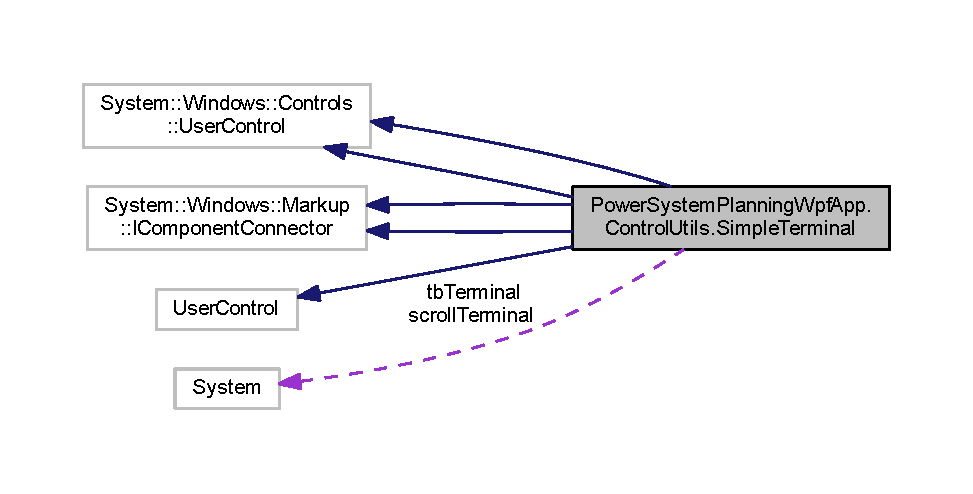
\includegraphics[width=350pt]{class_power_system_planning_wpf_app_1_1_control_utils_1_1_simple_terminal__coll__graph}
\end{center}
\end{figure}
\subsection*{Public Member Functions}
\begin{DoxyCompactItemize}
\item 
void {\bfseries Add\+Message\+To\+Terminal} (string message)\hypertarget{class_power_system_planning_wpf_app_1_1_control_utils_1_1_simple_terminal_a26cf665eb458128a13e724fdd54f4ec0}{}\label{class_power_system_planning_wpf_app_1_1_control_utils_1_1_simple_terminal_a26cf665eb458128a13e724fdd54f4ec0}

\item 
void \hyperlink{class_power_system_planning_wpf_app_1_1_control_utils_1_1_simple_terminal_a87d7756e060b71939deecee9453d1eac}{Initialize\+Component} ()
\begin{DoxyCompactList}\small\item\em Initialize\+Component \end{DoxyCompactList}\item 
void \hyperlink{class_power_system_planning_wpf_app_1_1_control_utils_1_1_simple_terminal_a87d7756e060b71939deecee9453d1eac}{Initialize\+Component} ()
\begin{DoxyCompactList}\small\item\em Initialize\+Component \end{DoxyCompactList}\end{DoxyCompactItemize}
\subsection*{Properties}
\begin{DoxyCompactItemize}
\item 
double {\bfseries Scroll\+Height}\hspace{0.3cm}{\ttfamily  \mbox{[}get, set\mbox{]}}\hypertarget{class_power_system_planning_wpf_app_1_1_control_utils_1_1_simple_terminal_ae5f720d73de5ccec6fb9cf1780fa52dc}{}\label{class_power_system_planning_wpf_app_1_1_control_utils_1_1_simple_terminal_ae5f720d73de5ccec6fb9cf1780fa52dc}

\end{DoxyCompactItemize}


\subsection{Detailed Description}
Interaction logic for Simple\+Terminal.\+xaml 

\hyperlink{class_power_system_planning_wpf_app_1_1_control_utils_1_1_simple_terminal}{Simple\+Terminal} 

\subsection{Member Function Documentation}
\index{Power\+System\+Planning\+Wpf\+App\+::\+Control\+Utils\+::\+Simple\+Terminal@{Power\+System\+Planning\+Wpf\+App\+::\+Control\+Utils\+::\+Simple\+Terminal}!Initialize\+Component@{Initialize\+Component}}
\index{Initialize\+Component@{Initialize\+Component}!Power\+System\+Planning\+Wpf\+App\+::\+Control\+Utils\+::\+Simple\+Terminal@{Power\+System\+Planning\+Wpf\+App\+::\+Control\+Utils\+::\+Simple\+Terminal}}
\subsubsection[{\texorpdfstring{Initialize\+Component()}{InitializeComponent()}}]{\setlength{\rightskip}{0pt plus 5cm}void Power\+System\+Planning\+Wpf\+App.\+Control\+Utils.\+Simple\+Terminal.\+Initialize\+Component (
\begin{DoxyParamCaption}
{}
\end{DoxyParamCaption}
)\hspace{0.3cm}{\ttfamily [inline]}}\hypertarget{class_power_system_planning_wpf_app_1_1_control_utils_1_1_simple_terminal_a87d7756e060b71939deecee9453d1eac}{}\label{class_power_system_planning_wpf_app_1_1_control_utils_1_1_simple_terminal_a87d7756e060b71939deecee9453d1eac}


Initialize\+Component 

\index{Power\+System\+Planning\+Wpf\+App\+::\+Control\+Utils\+::\+Simple\+Terminal@{Power\+System\+Planning\+Wpf\+App\+::\+Control\+Utils\+::\+Simple\+Terminal}!Initialize\+Component@{Initialize\+Component}}
\index{Initialize\+Component@{Initialize\+Component}!Power\+System\+Planning\+Wpf\+App\+::\+Control\+Utils\+::\+Simple\+Terminal@{Power\+System\+Planning\+Wpf\+App\+::\+Control\+Utils\+::\+Simple\+Terminal}}
\subsubsection[{\texorpdfstring{Initialize\+Component()}{InitializeComponent()}}]{\setlength{\rightskip}{0pt plus 5cm}void Power\+System\+Planning\+Wpf\+App.\+Control\+Utils.\+Simple\+Terminal.\+Initialize\+Component (
\begin{DoxyParamCaption}
{}
\end{DoxyParamCaption}
)\hspace{0.3cm}{\ttfamily [inline]}}\hypertarget{class_power_system_planning_wpf_app_1_1_control_utils_1_1_simple_terminal_a87d7756e060b71939deecee9453d1eac}{}\label{class_power_system_planning_wpf_app_1_1_control_utils_1_1_simple_terminal_a87d7756e060b71939deecee9453d1eac}


Initialize\+Component 



The documentation for this class was generated from the following files\+:\begin{DoxyCompactItemize}
\item 
Control\+Utils/Simple\+Terminal.\+xaml.\+cs\item 
obj/\+Debug/\+Control\+Utils/Simple\+Terminal.\+g.\+cs\item 
obj/\+Debug/\+Control\+Utils/Simple\+Terminal.\+g.\+i.\+cs\end{DoxyCompactItemize}

\input{class_power_system_planning_wpf_app_1_1_static_t_e_p_1_1_static_t_e_p_window}
\hypertarget{class_power_system_planning_wpf_app_1_1_control_utils_1_1_window_datagrid_test}{}\section{Power\+System\+Planning\+Wpf\+App.\+Control\+Utils.\+Window\+Datagrid\+Test Class Reference}
\label{class_power_system_planning_wpf_app_1_1_control_utils_1_1_window_datagrid_test}\index{Power\+System\+Planning\+Wpf\+App.\+Control\+Utils.\+Window\+Datagrid\+Test@{Power\+System\+Planning\+Wpf\+App.\+Control\+Utils.\+Window\+Datagrid\+Test}}


Interaction logic for Window\+Datagrid\+Test.\+xaml  




Inheritance diagram for Power\+System\+Planning\+Wpf\+App.\+Control\+Utils.\+Window\+Datagrid\+Test\+:\nopagebreak
\begin{figure}[H]
\begin{center}
\leavevmode
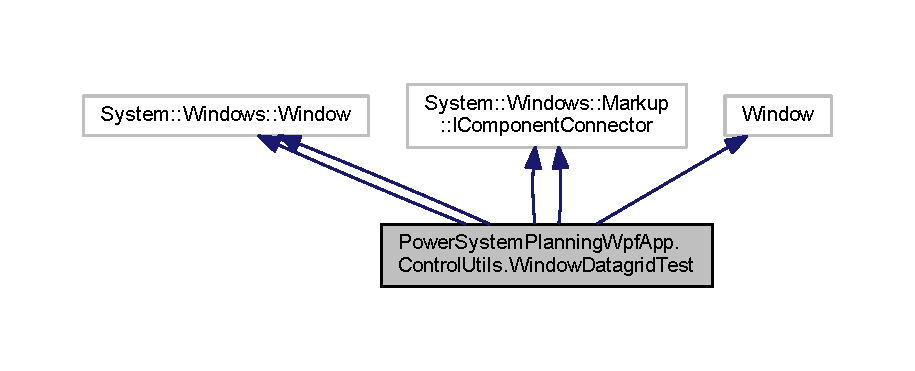
\includegraphics[width=350pt]{class_power_system_planning_wpf_app_1_1_control_utils_1_1_window_datagrid_test__inherit__graph}
\end{center}
\end{figure}


Collaboration diagram for Power\+System\+Planning\+Wpf\+App.\+Control\+Utils.\+Window\+Datagrid\+Test\+:\nopagebreak
\begin{figure}[H]
\begin{center}
\leavevmode
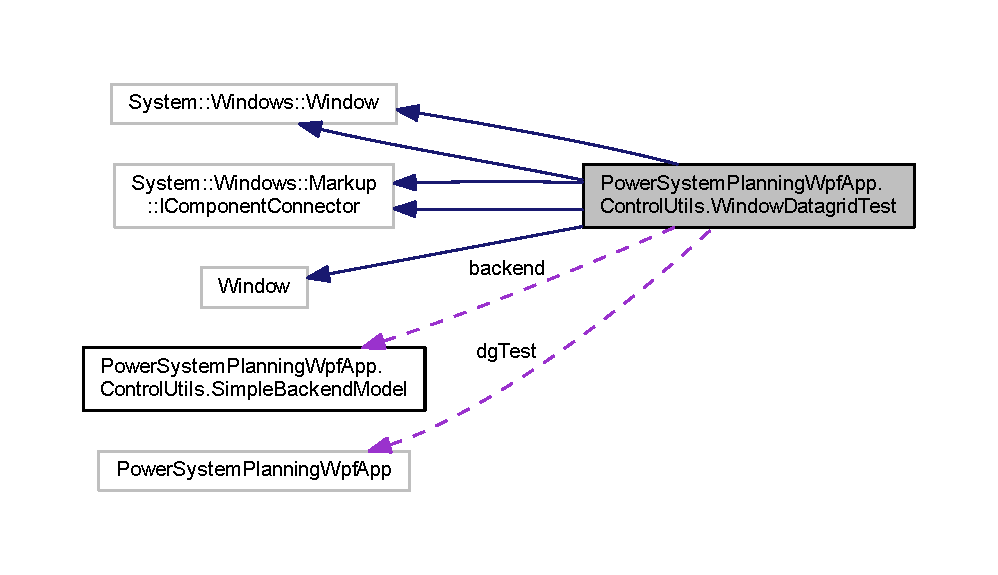
\includegraphics[width=350pt]{class_power_system_planning_wpf_app_1_1_control_utils_1_1_window_datagrid_test__coll__graph}
\end{center}
\end{figure}
\subsection*{Public Member Functions}
\begin{DoxyCompactItemize}
\item 
void \hyperlink{class_power_system_planning_wpf_app_1_1_control_utils_1_1_window_datagrid_test_a2ee573ee48c61c75d4817d43672b76b9}{Initialize\+Component} ()
\begin{DoxyCompactList}\small\item\em Initialize\+Component \end{DoxyCompactList}\item 
void \hyperlink{class_power_system_planning_wpf_app_1_1_control_utils_1_1_window_datagrid_test_a2ee573ee48c61c75d4817d43672b76b9}{Initialize\+Component} ()
\begin{DoxyCompactList}\small\item\em Initialize\+Component \end{DoxyCompactList}\end{DoxyCompactItemize}
\subsection*{Public Attributes}
\begin{DoxyCompactItemize}
\item 
\hyperlink{class_power_system_planning_wpf_app_1_1_control_utils_1_1_simple_backend_model}{Simple\+Backend\+Model} {\bfseries backend}\hypertarget{class_power_system_planning_wpf_app_1_1_control_utils_1_1_window_datagrid_test_a40b06d8fcd3574e8bdbfdd49086c0329}{}\label{class_power_system_planning_wpf_app_1_1_control_utils_1_1_window_datagrid_test_a40b06d8fcd3574e8bdbfdd49086c0329}

\end{DoxyCompactItemize}


\subsection{Detailed Description}
Interaction logic for Window\+Datagrid\+Test.\+xaml 

\hyperlink{class_power_system_planning_wpf_app_1_1_control_utils_1_1_window_datagrid_test}{Window\+Datagrid\+Test} 

\subsection{Member Function Documentation}
\index{Power\+System\+Planning\+Wpf\+App\+::\+Control\+Utils\+::\+Window\+Datagrid\+Test@{Power\+System\+Planning\+Wpf\+App\+::\+Control\+Utils\+::\+Window\+Datagrid\+Test}!Initialize\+Component@{Initialize\+Component}}
\index{Initialize\+Component@{Initialize\+Component}!Power\+System\+Planning\+Wpf\+App\+::\+Control\+Utils\+::\+Window\+Datagrid\+Test@{Power\+System\+Planning\+Wpf\+App\+::\+Control\+Utils\+::\+Window\+Datagrid\+Test}}
\subsubsection[{\texorpdfstring{Initialize\+Component()}{InitializeComponent()}}]{\setlength{\rightskip}{0pt plus 5cm}void Power\+System\+Planning\+Wpf\+App.\+Control\+Utils.\+Window\+Datagrid\+Test.\+Initialize\+Component (
\begin{DoxyParamCaption}
{}
\end{DoxyParamCaption}
)\hspace{0.3cm}{\ttfamily [inline]}}\hypertarget{class_power_system_planning_wpf_app_1_1_control_utils_1_1_window_datagrid_test_a2ee573ee48c61c75d4817d43672b76b9}{}\label{class_power_system_planning_wpf_app_1_1_control_utils_1_1_window_datagrid_test_a2ee573ee48c61c75d4817d43672b76b9}


Initialize\+Component 

\index{Power\+System\+Planning\+Wpf\+App\+::\+Control\+Utils\+::\+Window\+Datagrid\+Test@{Power\+System\+Planning\+Wpf\+App\+::\+Control\+Utils\+::\+Window\+Datagrid\+Test}!Initialize\+Component@{Initialize\+Component}}
\index{Initialize\+Component@{Initialize\+Component}!Power\+System\+Planning\+Wpf\+App\+::\+Control\+Utils\+::\+Window\+Datagrid\+Test@{Power\+System\+Planning\+Wpf\+App\+::\+Control\+Utils\+::\+Window\+Datagrid\+Test}}
\subsubsection[{\texorpdfstring{Initialize\+Component()}{InitializeComponent()}}]{\setlength{\rightskip}{0pt plus 5cm}void Power\+System\+Planning\+Wpf\+App.\+Control\+Utils.\+Window\+Datagrid\+Test.\+Initialize\+Component (
\begin{DoxyParamCaption}
{}
\end{DoxyParamCaption}
)\hspace{0.3cm}{\ttfamily [inline]}}\hypertarget{class_power_system_planning_wpf_app_1_1_control_utils_1_1_window_datagrid_test_a2ee573ee48c61c75d4817d43672b76b9}{}\label{class_power_system_planning_wpf_app_1_1_control_utils_1_1_window_datagrid_test_a2ee573ee48c61c75d4817d43672b76b9}


Initialize\+Component 



The documentation for this class was generated from the following files\+:\begin{DoxyCompactItemize}
\item 
Control\+Utils/Window\+Datagrid\+Test.\+xaml.\+cs\item 
obj/\+Debug/\+Control\+Utils/Window\+Datagrid\+Test.\+g.\+cs\item 
obj/\+Debug/\+Control\+Utils/Window\+Datagrid\+Test.\+g.\+i.\+cs\end{DoxyCompactItemize}

\hypertarget{class_power_system_planning_wpf_app_1_1_helper_1_1_wpf_rich_text_box_row_coloring_rule}{}\section{Power\+System\+Planning\+Wpf\+App.\+Helper.\+Wpf\+Rich\+Text\+Box\+Row\+Coloring\+Rule Class Reference}
\label{class_power_system_planning_wpf_app_1_1_helper_1_1_wpf_rich_text_box_row_coloring_rule}\index{Power\+System\+Planning\+Wpf\+App.\+Helper.\+Wpf\+Rich\+Text\+Box\+Row\+Coloring\+Rule@{Power\+System\+Planning\+Wpf\+App.\+Helper.\+Wpf\+Rich\+Text\+Box\+Row\+Coloring\+Rule}}
\subsection*{Public Member Functions}
\begin{DoxyCompactItemize}
\item 
{\bfseries Wpf\+Rich\+Text\+Box\+Row\+Coloring\+Rule} (string condition, string font\+Color, string back\+Color, Font\+Style font\+Style, Font\+Weight font\+Weight)\hypertarget{class_power_system_planning_wpf_app_1_1_helper_1_1_wpf_rich_text_box_row_coloring_rule_ae5180aeac6418aee6212ae92907ca948}{}\label{class_power_system_planning_wpf_app_1_1_helper_1_1_wpf_rich_text_box_row_coloring_rule_ae5180aeac6418aee6212ae92907ca948}

\item 
{\bfseries Wpf\+Rich\+Text\+Box\+Row\+Coloring\+Rule} (string condition, string font\+Color, string back\+Color)\hypertarget{class_power_system_planning_wpf_app_1_1_helper_1_1_wpf_rich_text_box_row_coloring_rule_aad529f4559f3adc3c9a092bb43fa5712}{}\label{class_power_system_planning_wpf_app_1_1_helper_1_1_wpf_rich_text_box_row_coloring_rule_aad529f4559f3adc3c9a092bb43fa5712}

\item 
bool {\bfseries Check\+Condition} (Log\+Event\+Info log\+Event)\hypertarget{class_power_system_planning_wpf_app_1_1_helper_1_1_wpf_rich_text_box_row_coloring_rule_ab6b52cc5cc7213fa6797dac3901dc6e1}{}\label{class_power_system_planning_wpf_app_1_1_helper_1_1_wpf_rich_text_box_row_coloring_rule_ab6b52cc5cc7213fa6797dac3901dc6e1}

\end{DoxyCompactItemize}
\subsection*{Properties}
\begin{DoxyCompactItemize}
\item 
static \hyperlink{class_power_system_planning_wpf_app_1_1_helper_1_1_wpf_rich_text_box_row_coloring_rule}{Wpf\+Rich\+Text\+Box\+Row\+Coloring\+Rule} {\bfseries Default}\hspace{0.3cm}{\ttfamily  \mbox{[}get\mbox{]}}\hypertarget{class_power_system_planning_wpf_app_1_1_helper_1_1_wpf_rich_text_box_row_coloring_rule_afb034e248d32994892e8a9543847b4d3}{}\label{class_power_system_planning_wpf_app_1_1_helper_1_1_wpf_rich_text_box_row_coloring_rule_afb034e248d32994892e8a9543847b4d3}

\item 
Condition\+Expression {\bfseries Condition}\hspace{0.3cm}{\ttfamily  \mbox{[}get, set\mbox{]}}\hypertarget{class_power_system_planning_wpf_app_1_1_helper_1_1_wpf_rich_text_box_row_coloring_rule_a40fdf9300385ebbecbe754c817412b6b}{}\label{class_power_system_planning_wpf_app_1_1_helper_1_1_wpf_rich_text_box_row_coloring_rule_a40fdf9300385ebbecbe754c817412b6b}

\item 
string {\bfseries Font\+Color}\hspace{0.3cm}{\ttfamily  \mbox{[}get, set\mbox{]}}\hypertarget{class_power_system_planning_wpf_app_1_1_helper_1_1_wpf_rich_text_box_row_coloring_rule_aefe6ec99beaf4b5d925b1a86f1ae7fc6}{}\label{class_power_system_planning_wpf_app_1_1_helper_1_1_wpf_rich_text_box_row_coloring_rule_aefe6ec99beaf4b5d925b1a86f1ae7fc6}

\item 
string {\bfseries Background\+Color}\hspace{0.3cm}{\ttfamily  \mbox{[}get, set\mbox{]}}\hypertarget{class_power_system_planning_wpf_app_1_1_helper_1_1_wpf_rich_text_box_row_coloring_rule_abe2cf575d5aa706c349a1c08f1c79305}{}\label{class_power_system_planning_wpf_app_1_1_helper_1_1_wpf_rich_text_box_row_coloring_rule_abe2cf575d5aa706c349a1c08f1c79305}

\item 
Font\+Style {\bfseries Style}\hspace{0.3cm}{\ttfamily  \mbox{[}get, set\mbox{]}}\hypertarget{class_power_system_planning_wpf_app_1_1_helper_1_1_wpf_rich_text_box_row_coloring_rule_a5f89b139d56af72e2a1dd268298cb61e}{}\label{class_power_system_planning_wpf_app_1_1_helper_1_1_wpf_rich_text_box_row_coloring_rule_a5f89b139d56af72e2a1dd268298cb61e}

\item 
Font\+Weight {\bfseries Weight}\hspace{0.3cm}{\ttfamily  \mbox{[}get, set\mbox{]}}\hypertarget{class_power_system_planning_wpf_app_1_1_helper_1_1_wpf_rich_text_box_row_coloring_rule_ab84a480685c42f6e460536656eb2fec7}{}\label{class_power_system_planning_wpf_app_1_1_helper_1_1_wpf_rich_text_box_row_coloring_rule_ab84a480685c42f6e460536656eb2fec7}

\end{DoxyCompactItemize}


The documentation for this class was generated from the following file\+:\begin{DoxyCompactItemize}
\item 
Helper/Wpf\+Rich\+Text\+Box\+Row\+Coloring\+Rule.\+cs\end{DoxyCompactItemize}

\hypertarget{class_power_system_planning_wpf_app_1_1_helper_1_1_wpf_rich_text_box_target}{}\section{Power\+System\+Planning\+Wpf\+App.\+Helper.\+Wpf\+Rich\+Text\+Box\+Target Class Reference}
\label{class_power_system_planning_wpf_app_1_1_helper_1_1_wpf_rich_text_box_target}\index{Power\+System\+Planning\+Wpf\+App.\+Helper.\+Wpf\+Rich\+Text\+Box\+Target@{Power\+System\+Planning\+Wpf\+App.\+Helper.\+Wpf\+Rich\+Text\+Box\+Target}}


Inheritance diagram for Power\+System\+Planning\+Wpf\+App.\+Helper.\+Wpf\+Rich\+Text\+Box\+Target\+:\nopagebreak
\begin{figure}[H]
\begin{center}
\leavevmode
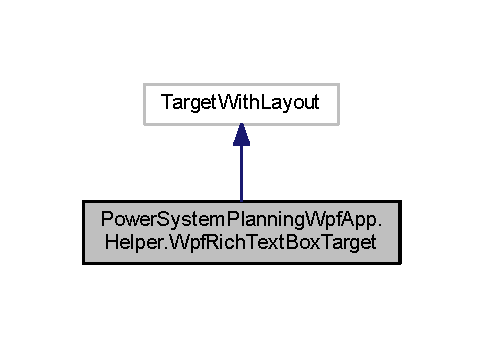
\includegraphics[width=232pt]{class_power_system_planning_wpf_app_1_1_helper_1_1_wpf_rich_text_box_target__inherit__graph}
\end{center}
\end{figure}


Collaboration diagram for Power\+System\+Planning\+Wpf\+App.\+Helper.\+Wpf\+Rich\+Text\+Box\+Target\+:\nopagebreak
\begin{figure}[H]
\begin{center}
\leavevmode
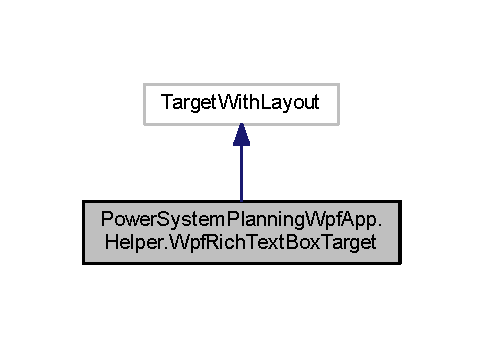
\includegraphics[width=232pt]{class_power_system_planning_wpf_app_1_1_helper_1_1_wpf_rich_text_box_target__coll__graph}
\end{center}
\end{figure}
\subsection*{Protected Member Functions}
\begin{DoxyCompactItemize}
\item 
override void {\bfseries Initialize\+Target} ()\hypertarget{class_power_system_planning_wpf_app_1_1_helper_1_1_wpf_rich_text_box_target_a92012c3bdfa4c3e9f59a951adedd14f9}{}\label{class_power_system_planning_wpf_app_1_1_helper_1_1_wpf_rich_text_box_target_a92012c3bdfa4c3e9f59a951adedd14f9}

\item 
override void {\bfseries Close\+Target} ()\hypertarget{class_power_system_planning_wpf_app_1_1_helper_1_1_wpf_rich_text_box_target_a1e3106334d793f1473c17f4a1d68023e}{}\label{class_power_system_planning_wpf_app_1_1_helper_1_1_wpf_rich_text_box_target_a1e3106334d793f1473c17f4a1d68023e}

\item 
override void {\bfseries Write} (Log\+Event\+Info log\+Event)\hypertarget{class_power_system_planning_wpf_app_1_1_helper_1_1_wpf_rich_text_box_target_a6a6ec9b0230077eed2c6b71822f32b98}{}\label{class_power_system_planning_wpf_app_1_1_helper_1_1_wpf_rich_text_box_target_a6a6ec9b0230077eed2c6b71822f32b98}

\end{DoxyCompactItemize}
\subsection*{Properties}
\begin{DoxyCompactItemize}
\item 
static Read\+Only\+Collection$<$ \hyperlink{class_power_system_planning_wpf_app_1_1_helper_1_1_wpf_rich_text_box_row_coloring_rule}{Wpf\+Rich\+Text\+Box\+Row\+Coloring\+Rule} $>$ {\bfseries Default\+Row\+Coloring\+Rules}\hspace{0.3cm}{\ttfamily  \mbox{[}get\mbox{]}}\hypertarget{class_power_system_planning_wpf_app_1_1_helper_1_1_wpf_rich_text_box_target_a12af7f68cd9b18eea4250828c668b3a6}{}\label{class_power_system_planning_wpf_app_1_1_helper_1_1_wpf_rich_text_box_target_a12af7f68cd9b18eea4250828c668b3a6}

\item 
string {\bfseries Control\+Name}\hspace{0.3cm}{\ttfamily  \mbox{[}get, set\mbox{]}}\hypertarget{class_power_system_planning_wpf_app_1_1_helper_1_1_wpf_rich_text_box_target_a780505a664466d84a8ec2b7b286454ef}{}\label{class_power_system_planning_wpf_app_1_1_helper_1_1_wpf_rich_text_box_target_a780505a664466d84a8ec2b7b286454ef}

\item 
string {\bfseries Form\+Name}\hspace{0.3cm}{\ttfamily  \mbox{[}get, set\mbox{]}}\hypertarget{class_power_system_planning_wpf_app_1_1_helper_1_1_wpf_rich_text_box_target_a85a08efd7484c91c55e75219e0640fc5}{}\label{class_power_system_planning_wpf_app_1_1_helper_1_1_wpf_rich_text_box_target_a85a08efd7484c91c55e75219e0640fc5}

\item 
bool {\bfseries Use\+Default\+Row\+Coloring\+Rules}\hspace{0.3cm}{\ttfamily  \mbox{[}get, set\mbox{]}}\hypertarget{class_power_system_planning_wpf_app_1_1_helper_1_1_wpf_rich_text_box_target_a4cdb7f5fc49d7bfe8af5be0b9669d8cf}{}\label{class_power_system_planning_wpf_app_1_1_helper_1_1_wpf_rich_text_box_target_a4cdb7f5fc49d7bfe8af5be0b9669d8cf}

\item 
I\+List$<$ \hyperlink{class_power_system_planning_wpf_app_1_1_helper_1_1_wpf_rich_text_box_row_coloring_rule}{Wpf\+Rich\+Text\+Box\+Row\+Coloring\+Rule} $>$ {\bfseries Row\+Coloring\+Rules}\hspace{0.3cm}{\ttfamily  \mbox{[}get\mbox{]}}\hypertarget{class_power_system_planning_wpf_app_1_1_helper_1_1_wpf_rich_text_box_target_a80644b87c8076868928f54d4bef865c3}{}\label{class_power_system_planning_wpf_app_1_1_helper_1_1_wpf_rich_text_box_target_a80644b87c8076868928f54d4bef865c3}

\item 
I\+List$<$ \hyperlink{class_power_system_planning_wpf_app_1_1_helper_1_1_wpf_rich_text_box_word_coloring_rule}{Wpf\+Rich\+Text\+Box\+Word\+Coloring\+Rule} $>$ {\bfseries Word\+Coloring\+Rules}\hspace{0.3cm}{\ttfamily  \mbox{[}get\mbox{]}}\hypertarget{class_power_system_planning_wpf_app_1_1_helper_1_1_wpf_rich_text_box_target_a0df68a584e4e683ca418c1ca2c6957e5}{}\label{class_power_system_planning_wpf_app_1_1_helper_1_1_wpf_rich_text_box_target_a0df68a584e4e683ca418c1ca2c6957e5}

\item 
bool {\bfseries Tool\+Window}\hspace{0.3cm}{\ttfamily  \mbox{[}get, set\mbox{]}}\hypertarget{class_power_system_planning_wpf_app_1_1_helper_1_1_wpf_rich_text_box_target_a5f907689f93312da593eaee205b6ebd5}{}\label{class_power_system_planning_wpf_app_1_1_helper_1_1_wpf_rich_text_box_target_a5f907689f93312da593eaee205b6ebd5}

\item 
bool {\bfseries Show\+Minimized}\hspace{0.3cm}{\ttfamily  \mbox{[}get, set\mbox{]}}\hypertarget{class_power_system_planning_wpf_app_1_1_helper_1_1_wpf_rich_text_box_target_a1cff1998a943c9c840302d01e3cedaa0}{}\label{class_power_system_planning_wpf_app_1_1_helper_1_1_wpf_rich_text_box_target_a1cff1998a943c9c840302d01e3cedaa0}

\item 
int {\bfseries Width}\hspace{0.3cm}{\ttfamily  \mbox{[}get, set\mbox{]}}\hypertarget{class_power_system_planning_wpf_app_1_1_helper_1_1_wpf_rich_text_box_target_ac28247a90b09fe912f65d9c115e17424}{}\label{class_power_system_planning_wpf_app_1_1_helper_1_1_wpf_rich_text_box_target_ac28247a90b09fe912f65d9c115e17424}

\item 
int {\bfseries Height}\hspace{0.3cm}{\ttfamily  \mbox{[}get, set\mbox{]}}\hypertarget{class_power_system_planning_wpf_app_1_1_helper_1_1_wpf_rich_text_box_target_abca99463301cb4b0378617a088c2579b}{}\label{class_power_system_planning_wpf_app_1_1_helper_1_1_wpf_rich_text_box_target_abca99463301cb4b0378617a088c2579b}

\item 
bool {\bfseries Auto\+Scroll}\hspace{0.3cm}{\ttfamily  \mbox{[}get, set\mbox{]}}\hypertarget{class_power_system_planning_wpf_app_1_1_helper_1_1_wpf_rich_text_box_target_a8505299ec7a8a0516f6664c5e744e9e1}{}\label{class_power_system_planning_wpf_app_1_1_helper_1_1_wpf_rich_text_box_target_a8505299ec7a8a0516f6664c5e744e9e1}

\item 
int {\bfseries Max\+Lines}\hspace{0.3cm}{\ttfamily  \mbox{[}get, set\mbox{]}}\hypertarget{class_power_system_planning_wpf_app_1_1_helper_1_1_wpf_rich_text_box_target_a0fa0becc053a1ce5e092b8aa6d53ae9c}{}\label{class_power_system_planning_wpf_app_1_1_helper_1_1_wpf_rich_text_box_target_a0fa0becc053a1ce5e092b8aa6d53ae9c}

\end{DoxyCompactItemize}


The documentation for this class was generated from the following file\+:\begin{DoxyCompactItemize}
\item 
Helper/Wpf\+Rich\+Text\+Box\+Target.\+cs\end{DoxyCompactItemize}

\hypertarget{class_power_system_planning_wpf_app_1_1_helper_1_1_wpf_rich_text_box_word_coloring_rule}{}\section{Power\+System\+Planning\+Wpf\+App.\+Helper.\+Wpf\+Rich\+Text\+Box\+Word\+Coloring\+Rule Class Reference}
\label{class_power_system_planning_wpf_app_1_1_helper_1_1_wpf_rich_text_box_word_coloring_rule}\index{Power\+System\+Planning\+Wpf\+App.\+Helper.\+Wpf\+Rich\+Text\+Box\+Word\+Coloring\+Rule@{Power\+System\+Planning\+Wpf\+App.\+Helper.\+Wpf\+Rich\+Text\+Box\+Word\+Coloring\+Rule}}
\subsection*{Public Member Functions}
\begin{DoxyCompactItemize}
\item 
{\bfseries Wpf\+Rich\+Text\+Box\+Word\+Coloring\+Rule} (string text, string font\+Color, string background\+Color)\hypertarget{class_power_system_planning_wpf_app_1_1_helper_1_1_wpf_rich_text_box_word_coloring_rule_a95c6ee034631b448b85ab4999bc4722a}{}\label{class_power_system_planning_wpf_app_1_1_helper_1_1_wpf_rich_text_box_word_coloring_rule_a95c6ee034631b448b85ab4999bc4722a}

\item 
{\bfseries Wpf\+Rich\+Text\+Box\+Word\+Coloring\+Rule} (string text, string text\+Color, string background\+Color, Font\+Style font\+Style, Font\+Weight font\+Weight)\hypertarget{class_power_system_planning_wpf_app_1_1_helper_1_1_wpf_rich_text_box_word_coloring_rule_a252dba951869aab9804d41d34c8d03b0}{}\label{class_power_system_planning_wpf_app_1_1_helper_1_1_wpf_rich_text_box_word_coloring_rule_a252dba951869aab9804d41d34c8d03b0}

\end{DoxyCompactItemize}
\subsection*{Properties}
\begin{DoxyCompactItemize}
\item 
string {\bfseries Regex}\hspace{0.3cm}{\ttfamily  \mbox{[}get, set\mbox{]}}\hypertarget{class_power_system_planning_wpf_app_1_1_helper_1_1_wpf_rich_text_box_word_coloring_rule_ae3c5500cc68010c2c42011a77edeccd9}{}\label{class_power_system_planning_wpf_app_1_1_helper_1_1_wpf_rich_text_box_word_coloring_rule_ae3c5500cc68010c2c42011a77edeccd9}

\item 
string {\bfseries Text}\hspace{0.3cm}{\ttfamily  \mbox{[}get, set\mbox{]}}\hypertarget{class_power_system_planning_wpf_app_1_1_helper_1_1_wpf_rich_text_box_word_coloring_rule_ab8d22f3298ea95b9d29484a4ef670159}{}\label{class_power_system_planning_wpf_app_1_1_helper_1_1_wpf_rich_text_box_word_coloring_rule_ab8d22f3298ea95b9d29484a4ef670159}

\item 
bool {\bfseries Whole\+Words}\hspace{0.3cm}{\ttfamily  \mbox{[}get, set\mbox{]}}\hypertarget{class_power_system_planning_wpf_app_1_1_helper_1_1_wpf_rich_text_box_word_coloring_rule_a5ed50d3aec5c16be24997b550842dc8a}{}\label{class_power_system_planning_wpf_app_1_1_helper_1_1_wpf_rich_text_box_word_coloring_rule_a5ed50d3aec5c16be24997b550842dc8a}

\item 
bool {\bfseries Ignore\+Case}\hspace{0.3cm}{\ttfamily  \mbox{[}get, set\mbox{]}}\hypertarget{class_power_system_planning_wpf_app_1_1_helper_1_1_wpf_rich_text_box_word_coloring_rule_a21289f33c29920505804f8517bd59b95}{}\label{class_power_system_planning_wpf_app_1_1_helper_1_1_wpf_rich_text_box_word_coloring_rule_a21289f33c29920505804f8517bd59b95}

\item 
Font\+Style {\bfseries Style}\hspace{0.3cm}{\ttfamily  \mbox{[}get, set\mbox{]}}\hypertarget{class_power_system_planning_wpf_app_1_1_helper_1_1_wpf_rich_text_box_word_coloring_rule_ac2582589b1650e531f4fb7a681004991}{}\label{class_power_system_planning_wpf_app_1_1_helper_1_1_wpf_rich_text_box_word_coloring_rule_ac2582589b1650e531f4fb7a681004991}

\item 
Font\+Weight {\bfseries Weight}\hspace{0.3cm}{\ttfamily  \mbox{[}get, set\mbox{]}}\hypertarget{class_power_system_planning_wpf_app_1_1_helper_1_1_wpf_rich_text_box_word_coloring_rule_a0e3994f1b167f708211e73c15e4392ab}{}\label{class_power_system_planning_wpf_app_1_1_helper_1_1_wpf_rich_text_box_word_coloring_rule_a0e3994f1b167f708211e73c15e4392ab}

\item 
Regex {\bfseries Compiled\+Regex}\hspace{0.3cm}{\ttfamily  \mbox{[}get\mbox{]}}\hypertarget{class_power_system_planning_wpf_app_1_1_helper_1_1_wpf_rich_text_box_word_coloring_rule_a2704d15e4f84518b1db231c27778feeb}{}\label{class_power_system_planning_wpf_app_1_1_helper_1_1_wpf_rich_text_box_word_coloring_rule_a2704d15e4f84518b1db231c27778feeb}

\item 
string {\bfseries Font\+Color}\hspace{0.3cm}{\ttfamily  \mbox{[}get, set\mbox{]}}\hypertarget{class_power_system_planning_wpf_app_1_1_helper_1_1_wpf_rich_text_box_word_coloring_rule_a0ed8792f2bfcf32484a6d5cbebdd601f}{}\label{class_power_system_planning_wpf_app_1_1_helper_1_1_wpf_rich_text_box_word_coloring_rule_a0ed8792f2bfcf32484a6d5cbebdd601f}

\item 
string {\bfseries Background\+Color}\hspace{0.3cm}{\ttfamily  \mbox{[}get, set\mbox{]}}\hypertarget{class_power_system_planning_wpf_app_1_1_helper_1_1_wpf_rich_text_box_word_coloring_rule_a5f01cf42d5bc69ba40eb635fd9cf8c2b}{}\label{class_power_system_planning_wpf_app_1_1_helper_1_1_wpf_rich_text_box_word_coloring_rule_a5f01cf42d5bc69ba40eb635fd9cf8c2b}

\end{DoxyCompactItemize}


The documentation for this class was generated from the following file\+:\begin{DoxyCompactItemize}
\item 
Helper/Wpf\+Rich\+Text\+Box\+Word\+Coloring\+Rule.\+cs\end{DoxyCompactItemize}

%--- End generated contents ---

% Index
\backmatter
\newpage
\phantomsection
\clearemptydoublepage
\addcontentsline{toc}{chapter}{Index}
\printindex

\end{document}
